%% bm.pdf preamble - material merged from previous preamble and current pandoc preamable output
% NOTE: float placement required changes to the source files referenced by bm.tex
% May 28, 2020
%
% Use lualatex to compile - test with MiKTeX 2.9

% uncomment to list all files in log
%\listfiles

\documentclass[12pt]{report}


\usepackage{fontspec}

%\setmainfont[Scale=MatchLowercase]{Lucida Bright}
%\setmonofont{FreeMono}
%\setmonofont{Source Code Pro}
\setmonofont[Scale=MatchLowercase]{Ubuntu Mono}

% short snippets of asian languages
\newfontfamily\myAsian{Noto Serif TC Medium}

\usepackage[headings]{fullpage}

% national use characters 
%\usepackage{inputenc}

% ams mathematical symbols
\usepackage{amsmath,amssymb}

% added to support pandoc highlighting
\usepackage{microtype}

\usepackage{makeidx}

% add index and bibliographies to table of contents
\usepackage[nottoc]{tocbibind}

% postscript courier and times in place of cm fonts
%\usepackage{courier}
%\usepackage{times}

% extended coloring
\usepackage{color}
\usepackage[table,dvipsnames]{xcolor}
\usepackage{colortbl}

% advanced date formating
\usepackage{datetime}

%support pandoc code highlighting
\usepackage{fancyvrb}

% \DefineShortVerb[commandchars=\\\{\}]{\|}
% \DefineVerbatimEnvironment{Highlighting}{Verbatim}{commandchars=\\\{\}}
% % Add ',fontsize=\small' for more characters per line

% tango style colors
% \usepackage{framed}
% \definecolor{shadecolor}{RGB}{255,255,255}
% \newenvironment{Shaded}{\begin{snugshade}}{\end{snugshade}}
% \newcommand{\KeywordTok}[1]{\textcolor[rgb]{0.13,0.29,0.53}{\textbf{{#1}}}}
% \newcommand{\DataTypeTok}[1]{\textcolor[rgb]{0.13,0.29,0.53}{{#1}}}
% \newcommand{\DecValTok}[1]{\textcolor[rgb]{0.00,0.00,0.81}{{#1}}}
% \newcommand{\BaseNTok}[1]{\textcolor[rgb]{0.00,0.00,0.81}{{#1}}}
% \newcommand{\FloatTok}[1]{\textcolor[rgb]{0.00,0.00,0.81}{{#1}}}
% \newcommand{\CharTok}[1]{\textcolor[rgb]{0.31,0.60,0.02}{{#1}}}
% \newcommand{\StringTok}[1]{\textcolor[rgb]{0.31,0.60,0.02}{{#1}}}
% \newcommand{\CommentTok}[1]{\textcolor[rgb]{0.56,0.35,0.01}{\textit{{#1}}}}
% \newcommand{\OtherTok}[1]{\textcolor[rgb]{0.56,0.35,0.01}{{#1}}}
% \newcommand{\AlertTok}[1]{\textcolor[rgb]{0.94,0.16,0.16}{{#1}}}
% \newcommand{\FunctionTok}[1]{\textcolor[rgb]{0.00,0.00,0.00}{{#1}}}
% \newcommand{\RegionMarkerTok}[1]{{#1}}
% \newcommand{\ErrorTok}[1]{\textbf{{#1}}}
% \newcommand{\NormalTok}[1]{{#1}}

% %espresso style colors
% \usepackage{framed}
% \definecolor{shadecolor}{RGB}{42,33,28}
% \newenvironment{Shaded}{\begin{snugshade}}{\end{snugshade}}
% \newcommand{\KeywordTok}[1]{\textcolor[rgb]{0.26,0.66,0.93}{\textbf{{#1}}}}
% \newcommand{\DataTypeTok}[1]{\textcolor[rgb]{0.74,0.68,0.62}{\underline{{#1}}}}
% \newcommand{\DecValTok}[1]{\textcolor[rgb]{0.27,0.67,0.26}{{#1}}}
% \newcommand{\BaseNTok}[1]{\textcolor[rgb]{0.27,0.67,0.26}{{#1}}}
% \newcommand{\FloatTok}[1]{\textcolor[rgb]{0.27,0.67,0.26}{{#1}}}
% \newcommand{\CharTok}[1]{\textcolor[rgb]{0.02,0.61,0.04}{{#1}}}
% \newcommand{\StringTok}[1]{\textcolor[rgb]{0.02,0.61,0.04}{{#1}}}
% \newcommand{\CommentTok}[1]{\textcolor[rgb]{0.00,0.40,1.00}{\textit{{#1}}}}
% \newcommand{\OtherTok}[1]{\textcolor[rgb]{0.74,0.68,0.62}{{#1}}}
% \newcommand{\AlertTok}[1]{\textcolor[rgb]{1.00,1.00,0.00}{{#1}}}
% \newcommand{\FunctionTok}[1]{\textcolor[rgb]{1.00,0.58,0.35}{\textbf{{#1}}}}
% \newcommand{\RegionMarkerTok}[1]{\textcolor[rgb]{0.74,0.68,0.62}{{#1}}}
% \newcommand{\ErrorTok}[1]{\textcolor[rgb]{0.74,0.68,0.62}{\textbf{{#1}}}}
% \newcommand{\NormalTok}[1]{\textcolor[rgb]{0.74,0.68,0.62}{{#1}}}

% %kete style colors
% \newenvironment{Shaded}{}{}
% \newcommand{\KeywordTok}[1]{\textbf{{#1}}}
% \newcommand{\DataTypeTok}[1]{\textcolor[rgb]{0.50,0.00,0.00}{{#1}}}
% \newcommand{\DecValTok}[1]{\textcolor[rgb]{0.00,0.00,1.00}{{#1}}}
% \newcommand{\BaseNTok}[1]{\textcolor[rgb]{0.00,0.00,1.00}{{#1}}}
% \newcommand{\FloatTok}[1]{\textcolor[rgb]{0.50,0.00,0.50}{{#1}}}
% \newcommand{\CharTok}[1]{\textcolor[rgb]{1.00,0.00,1.00}{{#1}}}
% \newcommand{\StringTok}[1]{\textcolor[rgb]{0.87,0.00,0.00}{{#1}}}
% \newcommand{\CommentTok}[1]{\textcolor[rgb]{0.50,0.50,0.50}{\textit{{#1}}}}
% \newcommand{\OtherTok}[1]{{#1}}
% \newcommand{\AlertTok}[1]{\textcolor[rgb]{0.00,1.00,0.00}{\textbf{{#1}}}}
% \newcommand{\FunctionTok}[1]{\textcolor[rgb]{0.00,0.00,0.50}{{#1}}}
% \newcommand{\RegionMarkerTok}[1]{{#1}}
% \newcommand{\ErrorTok}[1]{\textcolor[rgb]{1.00,0.00,0.00}{\textbf{{#1}}}}
% \newcommand{\NormalTok}[1]{{#1}}
% %end pandoc code hacks

% jodliterate colors
\usepackage{color}
\definecolor{shadecolor}{RGB}{248,248,248}
% j control structures 
\definecolor{keywcolor}{rgb}{0.13,0.29,0.53}
% j explicit arguments x y m n u v
\definecolor{datacolor}{rgb}{0.13,0.29,0.53}
% j numbers - all types see j.xml
\definecolor{decvcolor}{rgb}{0.00,0.00,0.81}
\definecolor{basencolor}{rgb}{0.00,0.00,0.81}
\definecolor{floatcolor}{rgb}{0.00,0.00,0.81}
% j local assignments
\definecolor{charcolor}{rgb}{0.31,0.60,0.02}
\definecolor{stringcolor}{rgb}{0.31,0.60,0.02}
\definecolor{commentcolor}{rgb}{0.56,0.35,0.01}
% primitive adverbs and conjunctions
%\definecolor{othercolor}{rgb}{0.56,0.35,0.01}   
\definecolor{othercolor}{RGB}{0,0,255}
% global assignments
\definecolor{alertcolor}{rgb}{0.94,0.16,0.16}
% primitive J verbs and noun names
\definecolor{funccolor}{rgb}{0.00,0.00,0.00}

% custom colors
\definecolor{CodeBackGround}{cmyk}{0.0,0.0,0,0.05}    % light gray
\definecolor{CodeComment}{rgb}{0,0.50,0.00}           % dark green {0,0.45,0.08}
\definecolor{TableStripes}{gray}{0.9}                 % odd/even background in tables

% Colors for the hyperref package
\definecolor{urlcolor}{rgb}{0,.145,.698}
\definecolor{linkcolor}{rgb}{.71,0.21,0.01}
\definecolor{citecolor}{rgb}{.12,.54,.11}

% % Exact colors from NB
\definecolor{incolor}{HTML}{303F9F}
\definecolor{outcolor}{HTML}{D84315}
\definecolor{cellborder}{HTML}{CFCFCF}
\definecolor{cellbackground}{HTML}{F7F7F7}

% % ANSI colors
\definecolor{ansi-black}{HTML}{3E424D}
\definecolor{ansi-black-intense}{HTML}{282C36}
\definecolor{ansi-red}{HTML}{E75C58}
\definecolor{ansi-red-intense}{HTML}{B22B31}
\definecolor{ansi-green}{HTML}{00A250}
\definecolor{ansi-green-intense}{HTML}{007427}
\definecolor{ansi-yellow}{HTML}{DDB62B}
\definecolor{ansi-yellow-intense}{HTML}{B27D12}
\definecolor{ansi-blue}{HTML}{208FFB}
\definecolor{ansi-blue-intense}{HTML}{0065CA}
\definecolor{ansi-magenta}{HTML}{D160C4}
\definecolor{ansi-magenta-intense}{HTML}{A03196}
\definecolor{ansi-cyan}{HTML}{60C6C8}
\definecolor{ansi-cyan-intense}{HTML}{258F8F}
\definecolor{ansi-white}{HTML}{C5C1B4}
\definecolor{ansi-white-intense}{HTML}{A1A6B2}
\definecolor{ansi-default-inverse-fg}{HTML}{FFFFFF}
\definecolor{ansi-default-inverse-bg}{HTML}{000000}
    

% \usepackage{framed}
% \newenvironment{Shaded}{}{}
% \newcommand{\KeywordTok}[1]{\textcolor{keywcolor}{\textbf{{#1}}}}
% \newcommand{\DataTypeTok}[1]{\textcolor{datacolor}{{#1}}}
% %\newcommand{\DecValTok}[1]{\textcolor{decvcolor}{{#1}}}
% \newcommand{\DecValTok}[1]{{#1}} 
% \newcommand{\BaseNTok}[1]{\textcolor{basencolor}{{#1}}}
% \newcommand{\FloatTok}[1]{\textcolor{floatcolor}{{#1}}}
% \newcommand{\CharTok}[1]{\textcolor{charcolor}{\textbf{{#1}}}}
% \newcommand{\StringTok}[1]{\textcolor{stringcolor}{{#1}}}
% \newcommand{\CommentTok}[1]{\textcolor{commentcolor}{\textit{{#1}}}}
% \newcommand{\OtherTok}[1]{\textcolor{othercolor}{{#1}}} 
% \newcommand{\AlertTok}[1]{\textcolor{alertcolor}{\textbf{{#1}}}}
% %\newcommand{\FunctionTok}[1]{\textcolor{funccolor}{{#1}}}
% \newcommand{\FunctionTok}[1]{{#1}}
% \newcommand{\RegionMarkerTok}[1]{{#1}}
% \newcommand{\ErrorTok}[1]{\textbf{{#1}}}
% \newcommand{\NormalTok}[1]{{#1}}

% The default LaTeX title has an obnoxious amount of whitespace. By default,
% titling removes some of it. It also provides customization options.
\usepackage{titling}

% headers and footers
\usepackage{fancyhdr}
%\pagestyle{fancy}
\pagestyle{plain}

\fancyhead{}
\fancyfoot{}

%\fancyhead[LE,RO]{\slshape \rightmark}
%\fancyhead[LO,RE]{\slshape \leftmark}
\fancyfoot[C]{\thepage}
%\headrulewidth 0.4pt
%\footrulewidth 0 pt

%\addtolength{\headheight}{\baselineskip}

%\lfoot{\emph{Analyze the Data not the Drivel}}
%\rfoot{\emph{\today}}

% subfigure handles figures that contain subfigures
%\usepackage{color,graphicx,subfigure,sidecap}
\usepackage{graphicx,sidecap}
\usepackage{subfigure}
\graphicspath{{./inclusions/}}

% floatflt provides for text wrapping around small figures and tables
\usepackage{floatflt}

% tweak caption formats 
\usepackage{caption} 
\usepackage{sidecap}
%\usepackage{subcaption} % not compatible with subfigure

\usepackage{rotating} % flip tables sideways

% complex footnotes
%\usepackage{bigfoot}

% weird logos \XeLaTeX
\usepackage{metalogo}

\newcommand{\HRule}{\rule{\linewidth}{0.5mm}}

\usepackage[breakable]{tcolorbox}

\usepackage{parskip} % Stop auto-indenting (to mimic markdown behaviour)
    
% Basic figure setup, for now with no caption control since it's done
% automatically by Pandoc (which extracts ![](path) syntax from Markdown).
\usepackage{graphicx}

%\DeclareCaptionFormat{nocaption}{}
%\captionsetup{format=nocaption,aboveskip=0pt,belowskip=0pt}

\usepackage[Export]{adjustbox} % Used to constrain images to a maximum size
\adjustboxset{max size={0.9\linewidth}{0.9\paperheight}}
\usepackage{float}

%\floatplacement{figure}{H} % forces figures to be placed at the correct location

\usepackage{xcolor} % Allow colors to be defined
\usepackage{enumerate} % Needed for markdown enumerations to work
\usepackage{geometry} % Used to adjust the document margins

%\usepackage{amsmath} % Equations
%\usepackage{amssymb} % Equations

\usepackage{textcomp} % defines textquotesingle

% Hack from http://tex.stackexchange.com/a/47451/13684:
\AtBeginDocument{%
	\def\PYZsq{\textquotesingle}% Upright quotes in Pygmentized code
}

\usepackage{upquote} % Upright quotes for verbatim code
\usepackage{eurosym} % defines \euro
\usepackage[mathletters]{ucs} % Extended unicode (utf-8) support

%\usepackage{fancyvrb} % verbatim replacement that allows latex

\usepackage{grffile} % extends the file name processing of package graphics 
					 % to support a larger range
					 
\makeatletter % fix for grffile with XeLaTeX
\def\Gread@@xetex#1{%
  \IfFileExists{"\Gin@base".bb}%
  {\Gread@eps{\Gin@base.bb}}%
  {\Gread@@xetex@aux#1}%
}
\makeatother

% The hyperref package gives us a pdf with properly built
% internal navigation ('pdf bookmarks' for the table of contents,
% internal cross-reference links, web links for URLs, etc.)
\usepackage{hyperref}
% The default LaTeX title has an obnoxious amount of whitespace. By default,
% titling removes some of it. It also provides customization options.
\usepackage{titling}
\usepackage{longtable} % longtable support required by pandoc >1.10
\usepackage{booktabs}  % table support for pandoc > 1.12.2
\usepackage[inline]{enumitem} % IRkernel/repr support (it uses the enumerate* environment)
\usepackage[normalem]{ulem} % ulem is needed to support strikethroughs (\sout)
							% normalem makes italics be italics, not underlines
\usepackage{mathrsfs}

% commands and environments needed by pandoc snippets
% extracted from the output of `pandoc -s`
\providecommand{\tightlist}{%
  \setlength{\itemsep}{0pt}\setlength{\parskip}{0pt}}
  
\DefineVerbatimEnvironment{Highlighting}{Verbatim}{commandchars=\\\{\}}
% Add ',fontsize=\small' for more characters per line
\newenvironment{Shaded}{}{}
\newcommand{\KeywordTok}[1]{\textcolor[rgb]{0.00,0.44,0.13}{\textbf{{#1}}}}
\newcommand{\DataTypeTok}[1]{\textcolor[rgb]{0.56,0.13,0.00}{{#1}}}
\newcommand{\DecValTok}[1]{\textcolor[rgb]{0.25,0.63,0.44}{{#1}}}
\newcommand{\BaseNTok}[1]{\textcolor[rgb]{0.25,0.63,0.44}{{#1}}}
\newcommand{\FloatTok}[1]{\textcolor[rgb]{0.25,0.63,0.44}{{#1}}}
\newcommand{\CharTok}[1]{\textcolor[rgb]{0.25,0.44,0.63}{{#1}}}
\newcommand{\StringTok}[1]{\textcolor[rgb]{0.25,0.44,0.63}{{#1}}}
\newcommand{\CommentTok}[1]{\textcolor[rgb]{0.38,0.63,0.69}{\textit{{#1}}}}
\newcommand{\OtherTok}[1]{\textcolor[rgb]{0.00,0.44,0.13}{{#1}}}
\newcommand{\AlertTok}[1]{\textcolor[rgb]{1.00,0.00,0.00}{\textbf{{#1}}}}
\newcommand{\FunctionTok}[1]{\textcolor[rgb]{0.02,0.16,0.49}{{#1}}}
\newcommand{\RegionMarkerTok}[1]{{#1}}
\newcommand{\ErrorTok}[1]{\textcolor[rgb]{1.00,0.00,0.00}{\textbf{{#1}}}}
\newcommand{\NormalTok}[1]{{#1}}

% Additional commands for more recent versions of Pandoc
\newcommand{\ConstantTok}[1]{\textcolor[rgb]{0.53,0.00,0.00}{{#1}}}
\newcommand{\SpecialCharTok}[1]{\textcolor[rgb]{0.25,0.44,0.63}{{#1}}}
\newcommand{\VerbatimStringTok}[1]{\textcolor[rgb]{0.25,0.44,0.63}{{#1}}}
\newcommand{\SpecialStringTok}[1]{\textcolor[rgb]{0.73,0.40,0.53}{{#1}}}
\newcommand{\ImportTok}[1]{{#1}}
\newcommand{\DocumentationTok}[1]{\textcolor[rgb]{0.73,0.13,0.13}{\textit{{#1}}}}
\newcommand{\AnnotationTok}[1]{\textcolor[rgb]{0.38,0.63,0.69}{\textbf{\textit{{#1}}}}}
\newcommand{\CommentVarTok}[1]{\textcolor[rgb]{0.38,0.63,0.69}{\textbf{\textit{{#1}}}}}
\newcommand{\VariableTok}[1]{\textcolor[rgb]{0.10,0.09,0.49}{{#1}}}
\newcommand{\ControlFlowTok}[1]{\textcolor[rgb]{0.00,0.44,0.13}{\textbf{{#1}}}}
\newcommand{\OperatorTok}[1]{\textcolor[rgb]{0.40,0.40,0.40}{{#1}}}
\newcommand{\BuiltInTok}[1]{{#1}}
\newcommand{\ExtensionTok}[1]{{#1}}
\newcommand{\PreprocessorTok}[1]{\textcolor[rgb]{0.74,0.48,0.00}{{#1}}}
\newcommand{\AttributeTok}[1]{\textcolor[rgb]{0.49,0.56,0.16}{{#1}}}
\newcommand{\InformationTok}[1]{\textcolor[rgb]{0.38,0.63,0.69}{\textbf{\textit{{#1}}}}}
\newcommand{\WarningTok}[1]{\textcolor[rgb]{0.38,0.63,0.69}{\textbf{\textit{{#1}}}}}

% Define a nice break command that doesn't care if a line doesn't already exist.
\def\br{\hspace*{\fill} \\* }
% Math Jax compatibility definitions
\def\gt{>}
\def\lt{<}
\let\Oldtex\TeX
\let\Oldlatex\LaTeX
\renewcommand{\TeX}{\textrm{\Oldtex}}
\renewcommand{\LaTeX}{\textrm{\Oldlatex}}
 
% Pygments definitions
\makeatletter
\def\PY@reset{\let\PY@it=\relax \let\PY@bf=\relax%
    \let\PY@ul=\relax \let\PY@tc=\relax%
    \let\PY@bc=\relax \let\PY@ff=\relax}
\def\PY@tok#1{\csname PY@tok@#1\endcsname}
\def\PY@toks#1+{\ifx\relax#1\empty\else%
    \PY@tok{#1}\expandafter\PY@toks\fi}
\def\PY@do#1{\PY@bc{\PY@tc{\PY@ul{%
    \PY@it{\PY@bf{\PY@ff{#1}}}}}}}
\def\PY#1#2{\PY@reset\PY@toks#1+\relax+\PY@do{#2}}

\expandafter\def\csname PY@tok@w\endcsname{\def\PY@tc##1{\textcolor[rgb]{0.73,0.73,0.73}{##1}}}
\expandafter\def\csname PY@tok@c\endcsname{\let\PY@it=\textit\def\PY@tc##1{\textcolor[rgb]{0.25,0.50,0.50}{##1}}}
\expandafter\def\csname PY@tok@cp\endcsname{\def\PY@tc##1{\textcolor[rgb]{0.74,0.48,0.00}{##1}}}
\expandafter\def\csname PY@tok@k\endcsname{\let\PY@bf=\textbf\def\PY@tc##1{\textcolor[rgb]{0.00,0.50,0.00}{##1}}}
\expandafter\def\csname PY@tok@kp\endcsname{\def\PY@tc##1{\textcolor[rgb]{0.00,0.50,0.00}{##1}}}
\expandafter\def\csname PY@tok@kt\endcsname{\def\PY@tc##1{\textcolor[rgb]{0.69,0.00,0.25}{##1}}}
\expandafter\def\csname PY@tok@o\endcsname{\def\PY@tc##1{\textcolor[rgb]{0.40,0.40,0.40}{##1}}}
\expandafter\def\csname PY@tok@ow\endcsname{\let\PY@bf=\textbf\def\PY@tc##1{\textcolor[rgb]{0.67,0.13,1.00}{##1}}}
\expandafter\def\csname PY@tok@nb\endcsname{\def\PY@tc##1{\textcolor[rgb]{0.00,0.50,0.00}{##1}}}
\expandafter\def\csname PY@tok@nf\endcsname{\def\PY@tc##1{\textcolor[rgb]{0.00,0.00,1.00}{##1}}}
\expandafter\def\csname PY@tok@nc\endcsname{\let\PY@bf=\textbf\def\PY@tc##1{\textcolor[rgb]{0.00,0.00,1.00}{##1}}}
\expandafter\def\csname PY@tok@nn\endcsname{\let\PY@bf=\textbf\def\PY@tc##1{\textcolor[rgb]{0.00,0.00,1.00}{##1}}}
\expandafter\def\csname PY@tok@ne\endcsname{\let\PY@bf=\textbf\def\PY@tc##1{\textcolor[rgb]{0.82,0.25,0.23}{##1}}}
\expandafter\def\csname PY@tok@nv\endcsname{\def\PY@tc##1{\textcolor[rgb]{0.10,0.09,0.49}{##1}}}
\expandafter\def\csname PY@tok@no\endcsname{\def\PY@tc##1{\textcolor[rgb]{0.53,0.00,0.00}{##1}}}
\expandafter\def\csname PY@tok@nl\endcsname{\def\PY@tc##1{\textcolor[rgb]{0.63,0.63,0.00}{##1}}}
\expandafter\def\csname PY@tok@ni\endcsname{\let\PY@bf=\textbf\def\PY@tc##1{\textcolor[rgb]{0.60,0.60,0.60}{##1}}}
\expandafter\def\csname PY@tok@na\endcsname{\def\PY@tc##1{\textcolor[rgb]{0.49,0.56,0.16}{##1}}}
\expandafter\def\csname PY@tok@nt\endcsname{\let\PY@bf=\textbf\def\PY@tc##1{\textcolor[rgb]{0.00,0.50,0.00}{##1}}}
\expandafter\def\csname PY@tok@nd\endcsname{\def\PY@tc##1{\textcolor[rgb]{0.67,0.13,1.00}{##1}}}
\expandafter\def\csname PY@tok@s\endcsname{\def\PY@tc##1{\textcolor[rgb]{0.73,0.13,0.13}{##1}}}
\expandafter\def\csname PY@tok@sd\endcsname{\let\PY@it=\textit\def\PY@tc##1{\textcolor[rgb]{0.73,0.13,0.13}{##1}}}
\expandafter\def\csname PY@tok@si\endcsname{\let\PY@bf=\textbf\def\PY@tc##1{\textcolor[rgb]{0.73,0.40,0.53}{##1}}}
\expandafter\def\csname PY@tok@se\endcsname{\let\PY@bf=\textbf\def\PY@tc##1{\textcolor[rgb]{0.73,0.40,0.13}{##1}}}
\expandafter\def\csname PY@tok@sr\endcsname{\def\PY@tc##1{\textcolor[rgb]{0.73,0.40,0.53}{##1}}}
\expandafter\def\csname PY@tok@ss\endcsname{\def\PY@tc##1{\textcolor[rgb]{0.10,0.09,0.49}{##1}}}
\expandafter\def\csname PY@tok@sx\endcsname{\def\PY@tc##1{\textcolor[rgb]{0.00,0.50,0.00}{##1}}}
\expandafter\def\csname PY@tok@m\endcsname{\def\PY@tc##1{\textcolor[rgb]{0.40,0.40,0.40}{##1}}}
\expandafter\def\csname PY@tok@gh\endcsname{\let\PY@bf=\textbf\def\PY@tc##1{\textcolor[rgb]{0.00,0.00,0.50}{##1}}}
\expandafter\def\csname PY@tok@gu\endcsname{\let\PY@bf=\textbf\def\PY@tc##1{\textcolor[rgb]{0.50,0.00,0.50}{##1}}}
\expandafter\def\csname PY@tok@gd\endcsname{\def\PY@tc##1{\textcolor[rgb]{0.63,0.00,0.00}{##1}}}
\expandafter\def\csname PY@tok@gi\endcsname{\def\PY@tc##1{\textcolor[rgb]{0.00,0.63,0.00}{##1}}}
\expandafter\def\csname PY@tok@gr\endcsname{\def\PY@tc##1{\textcolor[rgb]{1.00,0.00,0.00}{##1}}}
\expandafter\def\csname PY@tok@ge\endcsname{\let\PY@it=\textit}
\expandafter\def\csname PY@tok@gs\endcsname{\let\PY@bf=\textbf}
\expandafter\def\csname PY@tok@gp\endcsname{\let\PY@bf=\textbf\def\PY@tc##1{\textcolor[rgb]{0.00,0.00,0.50}{##1}}}
\expandafter\def\csname PY@tok@go\endcsname{\def\PY@tc##1{\textcolor[rgb]{0.53,0.53,0.53}{##1}}}
\expandafter\def\csname PY@tok@gt\endcsname{\def\PY@tc##1{\textcolor[rgb]{0.00,0.27,0.87}{##1}}}
\expandafter\def\csname PY@tok@err\endcsname{\def\PY@bc##1{\setlength{\fboxsep}{0pt}\fcolorbox[rgb]{1.00,0.00,0.00}{1,1,1}{\strut ##1}}}
\expandafter\def\csname PY@tok@kc\endcsname{\let\PY@bf=\textbf\def\PY@tc##1{\textcolor[rgb]{0.00,0.50,0.00}{##1}}}
\expandafter\def\csname PY@tok@kd\endcsname{\let\PY@bf=\textbf\def\PY@tc##1{\textcolor[rgb]{0.00,0.50,0.00}{##1}}}
\expandafter\def\csname PY@tok@kn\endcsname{\let\PY@bf=\textbf\def\PY@tc##1{\textcolor[rgb]{0.00,0.50,0.00}{##1}}}
\expandafter\def\csname PY@tok@kr\endcsname{\let\PY@bf=\textbf\def\PY@tc##1{\textcolor[rgb]{0.00,0.50,0.00}{##1}}}
\expandafter\def\csname PY@tok@bp\endcsname{\def\PY@tc##1{\textcolor[rgb]{0.00,0.50,0.00}{##1}}}
\expandafter\def\csname PY@tok@fm\endcsname{\def\PY@tc##1{\textcolor[rgb]{0.00,0.00,1.00}{##1}}}
\expandafter\def\csname PY@tok@vc\endcsname{\def\PY@tc##1{\textcolor[rgb]{0.10,0.09,0.49}{##1}}}
\expandafter\def\csname PY@tok@vg\endcsname{\def\PY@tc##1{\textcolor[rgb]{0.10,0.09,0.49}{##1}}}
\expandafter\def\csname PY@tok@vi\endcsname{\def\PY@tc##1{\textcolor[rgb]{0.10,0.09,0.49}{##1}}}
\expandafter\def\csname PY@tok@vm\endcsname{\def\PY@tc##1{\textcolor[rgb]{0.10,0.09,0.49}{##1}}}
\expandafter\def\csname PY@tok@sa\endcsname{\def\PY@tc##1{\textcolor[rgb]{0.73,0.13,0.13}{##1}}}
\expandafter\def\csname PY@tok@sb\endcsname{\def\PY@tc##1{\textcolor[rgb]{0.73,0.13,0.13}{##1}}}
\expandafter\def\csname PY@tok@sc\endcsname{\def\PY@tc##1{\textcolor[rgb]{0.73,0.13,0.13}{##1}}}
\expandafter\def\csname PY@tok@dl\endcsname{\def\PY@tc##1{\textcolor[rgb]{0.73,0.13,0.13}{##1}}}
\expandafter\def\csname PY@tok@s2\endcsname{\def\PY@tc##1{\textcolor[rgb]{0.73,0.13,0.13}{##1}}}
\expandafter\def\csname PY@tok@sh\endcsname{\def\PY@tc##1{\textcolor[rgb]{0.73,0.13,0.13}{##1}}}
\expandafter\def\csname PY@tok@s1\endcsname{\def\PY@tc##1{\textcolor[rgb]{0.73,0.13,0.13}{##1}}}
\expandafter\def\csname PY@tok@mb\endcsname{\def\PY@tc##1{\textcolor[rgb]{0.40,0.40,0.40}{##1}}}
\expandafter\def\csname PY@tok@mf\endcsname{\def\PY@tc##1{\textcolor[rgb]{0.40,0.40,0.40}{##1}}}
\expandafter\def\csname PY@tok@mh\endcsname{\def\PY@tc##1{\textcolor[rgb]{0.40,0.40,0.40}{##1}}}
\expandafter\def\csname PY@tok@mi\endcsname{\def\PY@tc##1{\textcolor[rgb]{0.40,0.40,0.40}{##1}}}
\expandafter\def\csname PY@tok@il\endcsname{\def\PY@tc##1{\textcolor[rgb]{0.40,0.40,0.40}{##1}}}
\expandafter\def\csname PY@tok@mo\endcsname{\def\PY@tc##1{\textcolor[rgb]{0.40,0.40,0.40}{##1}}}
\expandafter\def\csname PY@tok@ch\endcsname{\let\PY@it=\textit\def\PY@tc##1{\textcolor[rgb]{0.25,0.50,0.50}{##1}}}
\expandafter\def\csname PY@tok@cm\endcsname{\let\PY@it=\textit\def\PY@tc##1{\textcolor[rgb]{0.25,0.50,0.50}{##1}}}
\expandafter\def\csname PY@tok@cpf\endcsname{\let\PY@it=\textit\def\PY@tc##1{\textcolor[rgb]{0.25,0.50,0.50}{##1}}}
\expandafter\def\csname PY@tok@c1\endcsname{\let\PY@it=\textit\def\PY@tc##1{\textcolor[rgb]{0.25,0.50,0.50}{##1}}}
\expandafter\def\csname PY@tok@cs\endcsname{\let\PY@it=\textit\def\PY@tc##1{\textcolor[rgb]{0.25,0.50,0.50}{##1}}}

\def\PYZbs{\char`\\}
\def\PYZus{\char`\_}
\def\PYZob{\char`\{}
\def\PYZcb{\char`\}}
\def\PYZca{\char`\^}
\def\PYZam{\char`\&}
\def\PYZlt{\char`\<}
\def\PYZgt{\char`\>}
\def\PYZsh{\char`\#}
\def\PYZpc{\char`\%}
\def\PYZdl{\char`\$}
\def\PYZhy{\char`\-}
\def\PYZsq{\char`\'}
\def\PYZdq{\char`\"}
\def\PYZti{\char`\~}
% for compatibility with earlier versions
\def\PYZat{@}
\def\PYZlb{[}
\def\PYZrb{]}
\makeatother

% For linebreaks inside Verbatim environment from package fancyvrb. 
\makeatletter
	\newbox\Wrappedcontinuationbox 
	\newbox\Wrappedvisiblespacebox 
	\newcommand*\Wrappedvisiblespace {\textcolor{red}{\textvisiblespace}} 
	\newcommand*\Wrappedcontinuationsymbol {\textcolor{red}{\llap{\tiny$\m@th\hookrightarrow$}}} 
	\newcommand*\Wrappedcontinuationindent {3ex } 
	\newcommand*\Wrappedafterbreak {\kern\Wrappedcontinuationindent\copy\Wrappedcontinuationbox} 
	% Take advantage of the already applied Pygments mark-up to insert 
	% potential linebreaks for TeX processing. 
	%        {, <, #, %, $, ' and ": go to next line. 
	%        _, }, ^, &, >, - and ~: stay at end of broken line. 
	% Use of \textquotesingle for straight quote. 
	\newcommand*\Wrappedbreaksatspecials {% 
		\def\PYGZus{\discretionary{\char`\_}{\Wrappedafterbreak}{\char`\_}}% 
		\def\PYGZob{\discretionary{}{\Wrappedafterbreak\char`\{}{\char`\{}}% 
		\def\PYGZcb{\discretionary{\char`\}}{\Wrappedafterbreak}{\char`\}}}% 
		\def\PYGZca{\discretionary{\char`\^}{\Wrappedafterbreak}{\char`\^}}% 
		\def\PYGZam{\discretionary{\char`\&}{\Wrappedafterbreak}{\char`\&}}% 
		\def\PYGZlt{\discretionary{}{\Wrappedafterbreak\char`\<}{\char`\<}}% 
		\def\PYGZgt{\discretionary{\char`\>}{\Wrappedafterbreak}{\char`\>}}% 
		\def\PYGZsh{\discretionary{}{\Wrappedafterbreak\char`\#}{\char`\#}}% 
		\def\PYGZpc{\discretionary{}{\Wrappedafterbreak\char`\%}{\char`\%}}% 
		\def\PYGZdl{\discretionary{}{\Wrappedafterbreak\char`\$}{\char`\$}}% 
		\def\PYGZhy{\discretionary{\char`\-}{\Wrappedafterbreak}{\char`\-}}% 
		\def\PYGZsq{\discretionary{}{\Wrappedafterbreak\textquotesingle}{\textquotesingle}}% 
		\def\PYGZdq{\discretionary{}{\Wrappedafterbreak\char`\"}{\char`\"}}% 
		\def\PYGZti{\discretionary{\char`\~}{\Wrappedafterbreak}{\char`\~}}% 
	} 
	% Some characters . , ; ? ! / are not pygmentized. 
	% This macro makes them "active" and they will insert potential linebreaks 
	\newcommand*\Wrappedbreaksatpunct {% 
		\lccode`\~`\.\lowercase{\def~}{\discretionary{\hbox{\char`\.}}{\Wrappedafterbreak}{\hbox{\char`\.}}}% 
		\lccode`\~`\,\lowercase{\def~}{\discretionary{\hbox{\char`\,}}{\Wrappedafterbreak}{\hbox{\char`\,}}}% 
		\lccode`\~`\;\lowercase{\def~}{\discretionary{\hbox{\char`\;}}{\Wrappedafterbreak}{\hbox{\char`\;}}}% 
		\lccode`\~`\:\lowercase{\def~}{\discretionary{\hbox{\char`\:}}{\Wrappedafterbreak}{\hbox{\char`\:}}}% 
		\lccode`\~`\?\lowercase{\def~}{\discretionary{\hbox{\char`\?}}{\Wrappedafterbreak}{\hbox{\char`\?}}}% 
		\lccode`\~`\!\lowercase{\def~}{\discretionary{\hbox{\char`\!}}{\Wrappedafterbreak}{\hbox{\char`\!}}}% 
		\lccode`\~`\/\lowercase{\def~}{\discretionary{\hbox{\char`\/}}{\Wrappedafterbreak}{\hbox{\char`\/}}}% 
		\catcode`\.\active
		\catcode`\,\active 
		\catcode`\;\active
		\catcode`\:\active
		\catcode`\?\active
		\catcode`\!\active
		\catcode`\/\active 
		\lccode`\~`\~ 	
	}
\makeatother

\let\OriginalVerbatim=\Verbatim
\makeatletter
\renewcommand{\Verbatim}[1][1]{%
	%\parskip\z@skip
	\sbox\Wrappedcontinuationbox {\Wrappedcontinuationsymbol}%
	\sbox\Wrappedvisiblespacebox {\FV@SetupFont\Wrappedvisiblespace}%
	\def\FancyVerbFormatLine ##1{\hsize\linewidth
		\vtop{\raggedright\hyphenpenalty\z@\exhyphenpenalty\z@
			\doublehyphendemerits\z@\finalhyphendemerits\z@
			\strut ##1\strut}%
	}%
	% If the linebreak is at a space, the latter will be displayed as visible
	% space at end of first line, and a continuation symbol starts next line.
	% Stretch/shrink are however usually zero for typewriter font.
	\def\FV@Space {%
		\nobreak\hskip\z@ plus\fontdimen3\font minus\fontdimen4\font
		\discretionary{\copy\Wrappedvisiblespacebox}{\Wrappedafterbreak}
		{\kern\fontdimen2\font}%
	}%
	
	% Allow breaks at special characters using \PYG... macros.
	\Wrappedbreaksatspecials
	% Breaks at punctuation characters . , ; ? ! and / need catcode=\active 	
	\OriginalVerbatim[#1,codes*=\Wrappedbreaksatpunct]%
}
\makeatother


% prompt
\makeatletter
\newcommand{\boxspacing}{\kern\kvtcb@left@rule\kern\kvtcb@boxsep}
\makeatother
\newcommand{\prompt}[4]{
	\ttfamily\llap{{\color{#2}[#3]:\hspace{3pt}#4}}\vspace{-\baselineskip}
}
    

% Prevent overflowing lines due to hard-to-break entities
\sloppy 

% Setup hyperref package
\hypersetup{
  breaklinks=true,  % so long urls are correctly broken across lines
  colorlinks=true,
  urlcolor=urlcolor,
  linkcolor=linkcolor,
  citecolor=citecolor,
  pdfauthor={John D. Baker},
  pdftitle={Analyze the Data not the Drivel},
  pdfsubject={Blog},
  pdfcreator={MikTeX+LaTeXe},
  pdfkeywords={blog,wordpress},
  }
  
% Slightly bigger margins than the latex defaults
% \geometry{verbose,tmargin=1in,bmargin=1in,lmargin=1in,rmargin=1in}  

%\usepackage{wrapfig}

% source code listings
\usepackage{listings}

\lstdefinelanguage{bat}
{morekeywords={echo,title,pushd,popd,setlocal,endlocal,off,if,not,exist,set,goto,pause},
sensitive=True,
morecomment=[l]{rem}
}

\lstdefinelanguage{jdoc}
{
morekeywords={},
otherkeywords={assert.,break.,continue.,for.,do.,if.,else.,elseif.,return.,select.,end.
,while.,whilst.,throw.,catch.,catchd.,catcht.,try.,case.,fcase.},
sensitive=True,
morecomment=[l]{NB.},
morestring=[b]',
morestring=[d]',
}

% latex size ordering - can never remember it
% \tiny
% \scriptsize
% \footnotesize
% \small
% \normalsize
% \large
% \Large
% \LARGE
% \huge
% \Huge
 
% listings package settings  
\lstset{%
  language=jdoc,                                % j document settings
  basicstyle=\ttfamily\footnotesize,            
  keywordstyle=\bfseries\color{keywcolor}\footnotesize,
  identifierstyle=\color{black},
  commentstyle=\slshape\color{CodeComment},     % colored slanted comments
  stringstyle=\color{red}\ttfamily,
  showstringspaces=false,                       
  %backgroundcolor=\color{CodeBackGround},       
  frame=single,                                
  framesep=1pt,                                 
  framerule=0.8pt,                             
  rulecolor=\color{CodeBackGround},   
  showspaces=false,
  %columns=fullflexible,
  %numbers=left,
  %numberstyle=\footnotesize,
  %numbersep=9pt,
  tabsize=2,
  showtabs=false,
  captionpos=b
  breaklines=true,                              
  breakindent=5pt                              
}

\lstdefinelanguage{JavaScript}{
  keywords={typeof, new, true, false, catch, function, return, null, catch, switch, var, if, in, while, do, else, case, break},
  ndkeywords={class, export, boolean, throw, implements, import, this},
  ndkeywordstyle=\color{darkgray}\bfseries,
  sensitive=false,
  comment=[l]{//},
  morecomment=[s]{/*}{*/},
  morestring=[b]',
  morestring=[b]"
}

% C# settings
\lstdefinestyle{sharpc}{
language=[Sharp]C,
basicstyle=\ttfamily\scriptsize, 
keywordstyle=\bfseries\color{keywcolor}\scriptsize,
framerule=0pt
}

% for source code listing longer than two use smaller font
\lstdefinestyle{smallersource}{
basicstyle=\ttfamily\scriptsize, 
keywordstyle=\bfseries\color{keywcolor}\scriptsize,
framerule=0pt
}

\lstdefinestyle{resetdefaults}{
language=jdoc,
basicstyle=\ttfamily\footnotesize,  
keywordstyle=\bfseries\color{keywcolor}\footnotesize,                                                               
framerule=0.8pt 
}

% APL UTF8 code points listed for lstlisting processing
\makeatletter
\lst@InputCatcodes
\def\lst@DefEC{%
 \lst@CCECUse \lst@ProcessLetter
  ^^80^^81^^82^^83^^84^^85^^86^^87^^88^^89^^8a^^8b^^8c^^8d^^8e^^8f%
  ^^90^^91^^92^^93^^94^^95^^96^^97^^98^^99^^9a^^9b^^9c^^9d^^9e^^9f%
  ^^a0^^a1^^a2^^a3^^a4^^a5^^a6^^a7^^a8^^a9^^aa^^ab^^ac^^ad^^ae^^af%
  ^^b0^^b1^^b2^^b3^^b4^^b5^^b6^^b7^^b8^^b9^^ba^^bb^^bc^^bd^^be^^bf%
  ^^c0^^c1^^c2^^c3^^c4^^c5^^c6^^c7^^c8^^c9^^ca^^cb^^cc^^cd^^ce^^cf%
  ^^d0^^d1^^d2^^d3^^d4^^d5^^d6^^d7^^d8^^d9^^da^^db^^dc^^dd^^de^^df%
  ^^e0^^e1^^e2^^e3^^e4^^e5^^e6^^e7^^e8^^e9^^ea^^eb^^ec^^ed^^ee^^ef%
  ^^f0^^f1^^f2^^f3^^f4^^f5^^f6^^f7^^f8^^f9^^fa^^fb^^fc^^fd^^fe^^ff%
  ^^^^20ac^^^^0153^^^^0152%
  ^^^^20a7^^^^2190^^^^2191^^^^2192^^^^2193^^^^2206^^^^2207^^^^220a%
  ^^^^2218^^^^2228^^^^2229^^^^222a^^^^2235^^^^223c^^^^2260^^^^2261%
  ^^^^2262^^^^2264^^^^2265^^^^2282^^^^2283^^^^2296^^^^22a2^^^^22a3%
  ^^^^22a4^^^^22a5^^^^22c4^^^^2308^^^^230a^^^^2336^^^^2337^^^^2339%
  ^^^^233b^^^^233d^^^^233f^^^^2340^^^^2342^^^^2347^^^^2348^^^^2349%
  ^^^^234b^^^^234e^^^^2350^^^^2352^^^^2355^^^^2357^^^^2359^^^^235d%
  ^^^^235e^^^^235f^^^^2361^^^^2362^^^^2363^^^^2364^^^^2365^^^^2368%
  ^^^^236a^^^^236b^^^^236c^^^^2371^^^^2372^^^^2373^^^^2374^^^^2375%
  ^^^^2377^^^^2378^^^^237a^^^^2395^^^^25af^^^^25ca^^^^25cb%  
  ^^00}
\lst@RestoreCatcodes
\makeatother

% custom lengths used within minipages
\newcommand{\minindent}{17pt}

\makeindex

\begin{document}

\subsection*{\href{https://analyzethedatanotthedrivel.org/2017/08/27/still-totally-awesome/}{Still Totally Awesome}}
\addcontentsline{toc}{subsection}{Still Totally Awesome}


\noindent\emph{Posted: 27 Aug 2017 20:36:53}
\vspace{6pt}

The total solar eclipse of August 21, 2017, was my fourth complete solar
eclipse. I've seen two annular eclipses, 1994 and 2012, and two total
eclipses, 2001 and 2017. Annular eclipses, or rings of fire, are worthy
spectacles but nothing compares to a total solar eclipse. Some things
have to be experienced to be fully appreciated. Unless you have stood
under the Moon's shadow you don't really know what it's like. Pictures
and recordings all miss the mark. Maybe one day, when virtual reality
directly hooks into all our senses, it may be possible to record
totality but until then you have to get under the Moon's shadow and,
this is absolutely crucial,~\emph{only totality counts!}

Here in the Boise Idaho area, many people decided 99\% was good enough.
This is not even wrong! The August 21\textsuperscript{st}~eclipse took
place right in the middle of Western Idaho State Fair and like all make
a buck opportunists the fair promoted an ``enjoy the eclipse with us
event.'' There was only one problem: Boise wasn't in the totality zone
so advertising dollars were spent reassuring fair-goers that 99\% was
close enough; that a measly 1\% difference was no big deal; that it
wasn't worth refraining from shoveling junk food down your obese
pie-hole on the overpriced midway. Cosmic spectacles cannot be allowed
to suppress the bottom line.

Fortunately, I knew better. The difference between 99\% and 100\% is
vast. Solar eclipse awesomeness is not linear! It's actually more like a
logarithmic step function with a really big step at totality. XKCD
accurately summarized this his with recent eclipse cartoon. He correctly
notes that total solar eclipses are off the scale.


%{[}caption id=``attachment\_5435'' align=``aligncenter''  width=``237''{]}
%\href{https://xkcd.com/1880/}{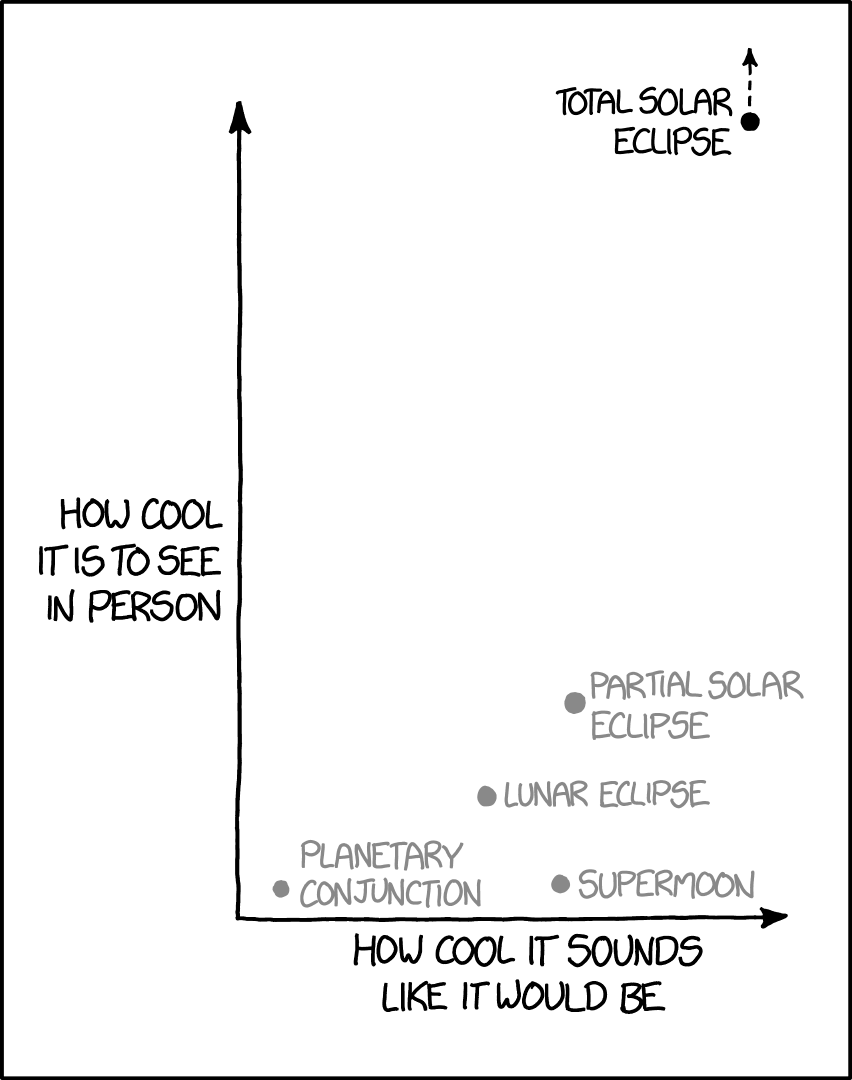
\includegraphics[width=2.46875in,height=3.12500in]{https://bakerjd99.files.wordpress.com/2017/08/eclipse_review.png?w=237}}
%XKCD accurately notes that total solar eclipse ``coolness'' is off the
%scale. Totality in on an entirely different plane than partial or
%annular eclipses.
%{[}/caption{]}

\captionsetup[figure]{labelformat=empty}

%\begin{figure}[htbp]
%\centering
%\href{https://xkcd.com/1880/}{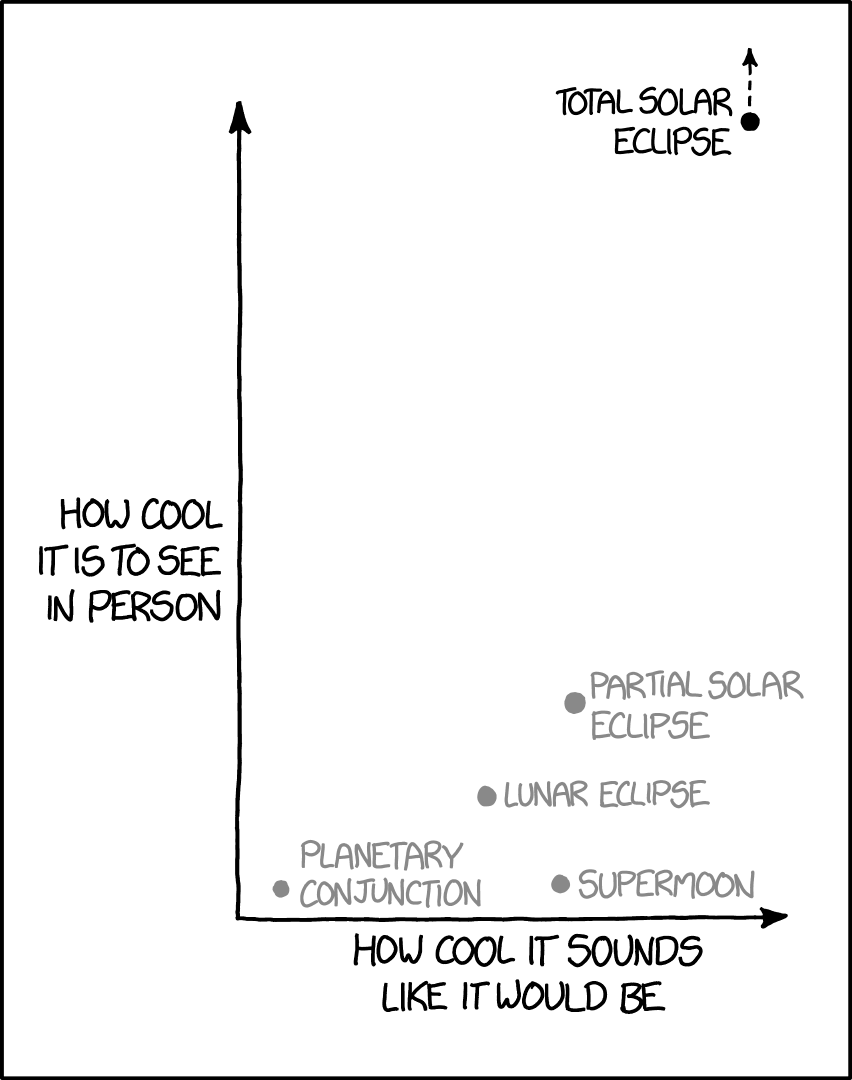
\includegraphics[width=0.50\textwidth]{eclipse_review.png}}
%\caption{XKCD accurately notes that total solar eclipse ``coolness'' is off the
%scale. Totality in on an entirely different plane than partial or
%annular eclipses.}
%\label{fig:5430x0}
%\end{figure}

\begin{SCfigure}[10]
\centering
\href{https://xkcd.com/1880/}{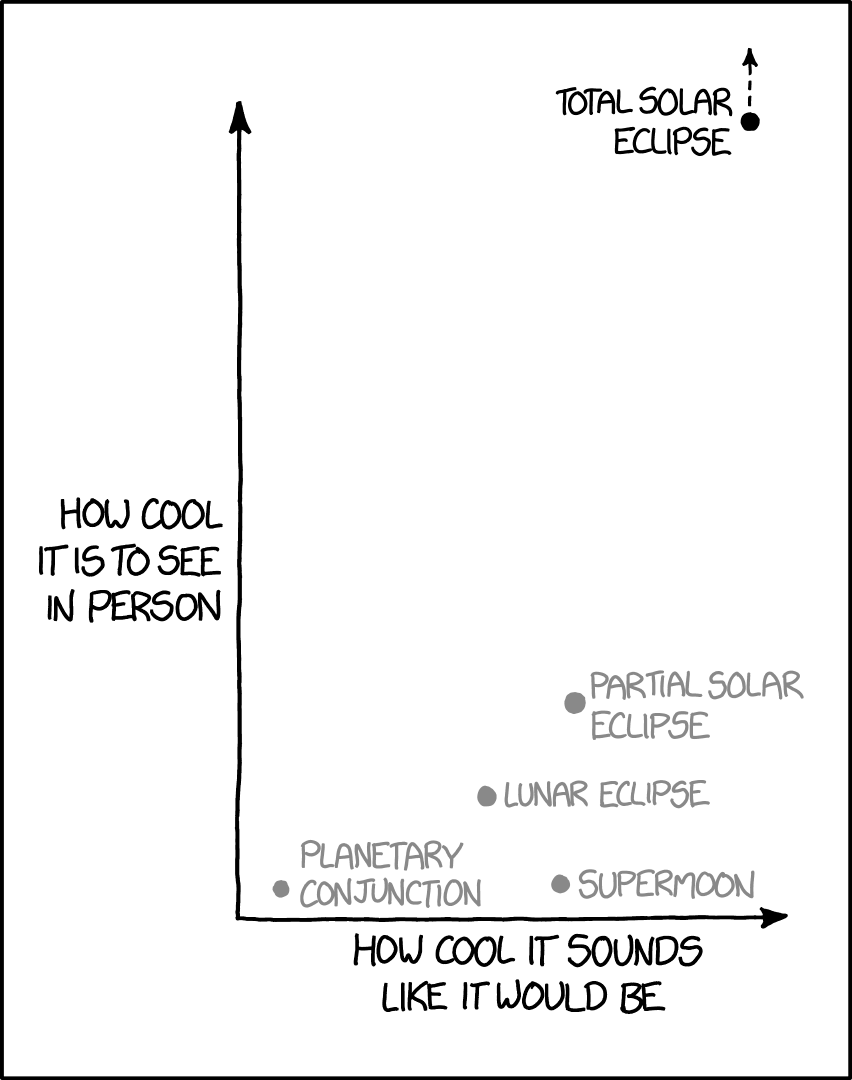
\includegraphics[width=0.38\textwidth]{eclipse_review.png}}
\caption{XKCD accurately notes that total solar eclipse ``coolness'' is off the
scale. Totality is on an entirely different plane than partial or
annular eclipses.}
\label{fig:5430x0}
\end{SCfigure}


There was no way I was going to miss totality, especially when it was
almost in my backyard, so we got up at 4:00 am on the
21\textsuperscript{st} and headed east to Mackay Idaho. I'd already
driven around southern Idaho and Oregon scouting eclipse watching
locations. My preferred location was on Sunset Peak in the Lost River
mountain range of Idaho. Unfortunately, Sunset Peak required that we
climb the mountain the night before, camp out near the summit, and then
wait for the eclipse the next morning. It would have been cool. Sunset
Peak is slightly over 3,050 meters with nice views to the west and east.
It would have been possible to watch the Moon's shadow race over the
Boise and Sawtooth mountains, blacking out one peak after another. I was
all ready to pack up and go but my wife no longer camps out in tents.
This is a problem I am still working on.

With the mountain summit vetoed we checked out the Snake River Valley
near Huntington Oregon and Stanley Idaho. Both locations are very scenic
but both required traversing easily congested roads. To ensure totality
we would have had to go the night before. So we were right back to
camping in tents. My third option Mackay Idaho was a nice mixture of,
easily reached on good roads, large enough to find parking on public
lands, and far enough out-of-the-way to avoid big crowds.

Mackay is about four hours from Meridian. To make it before first
contact, shortly after 10:00 am local time, and to miss projected heavy
traffic, we started at 4:00 am. In retrospect, we could have left later.
Traffic was light on I84 and almost nonexistent on Idaho highway 20. We
hardly saw another car until Highway 20 crossed the road to Sun Valley.
Sun Valley was in the totality zone but it was too far from the center
line for me. Leaving early paid off when we reached Craters of the Moon:
a smoke reddened Sun was creeping over the eastern horizon and
illuminating the black volcanic flows.


%{[}caption id=``attachment\_5440'' align=``aligncenter''  width=``500''{]}
%\href{https://conceptcontrol.smugmug.com/Places/USA-and-Canada/Idaho-Instants/i-mXNChFm/A}{\includegraphics[width=5.20833in,height=3.46875in]{https://bakerjd99.files.wordpress.com/2017/08/sunrise-craters-of-the-moon1.jpg?w=300}}
%We left Meridian at 4:00 am and headed east to Mackay Idaho to see the
%eclipse. On the way we caught the Sun rising over the Craters of the
%Moon. It was a good start to eclipse day.
%{[}/caption{]}

%\begin{figure}[htbp]
%\centering
%\href{https://conceptcontrol.smugmug.com/Places/USA-and-Canada/Idaho-Instants/i-mXNChFm/A}{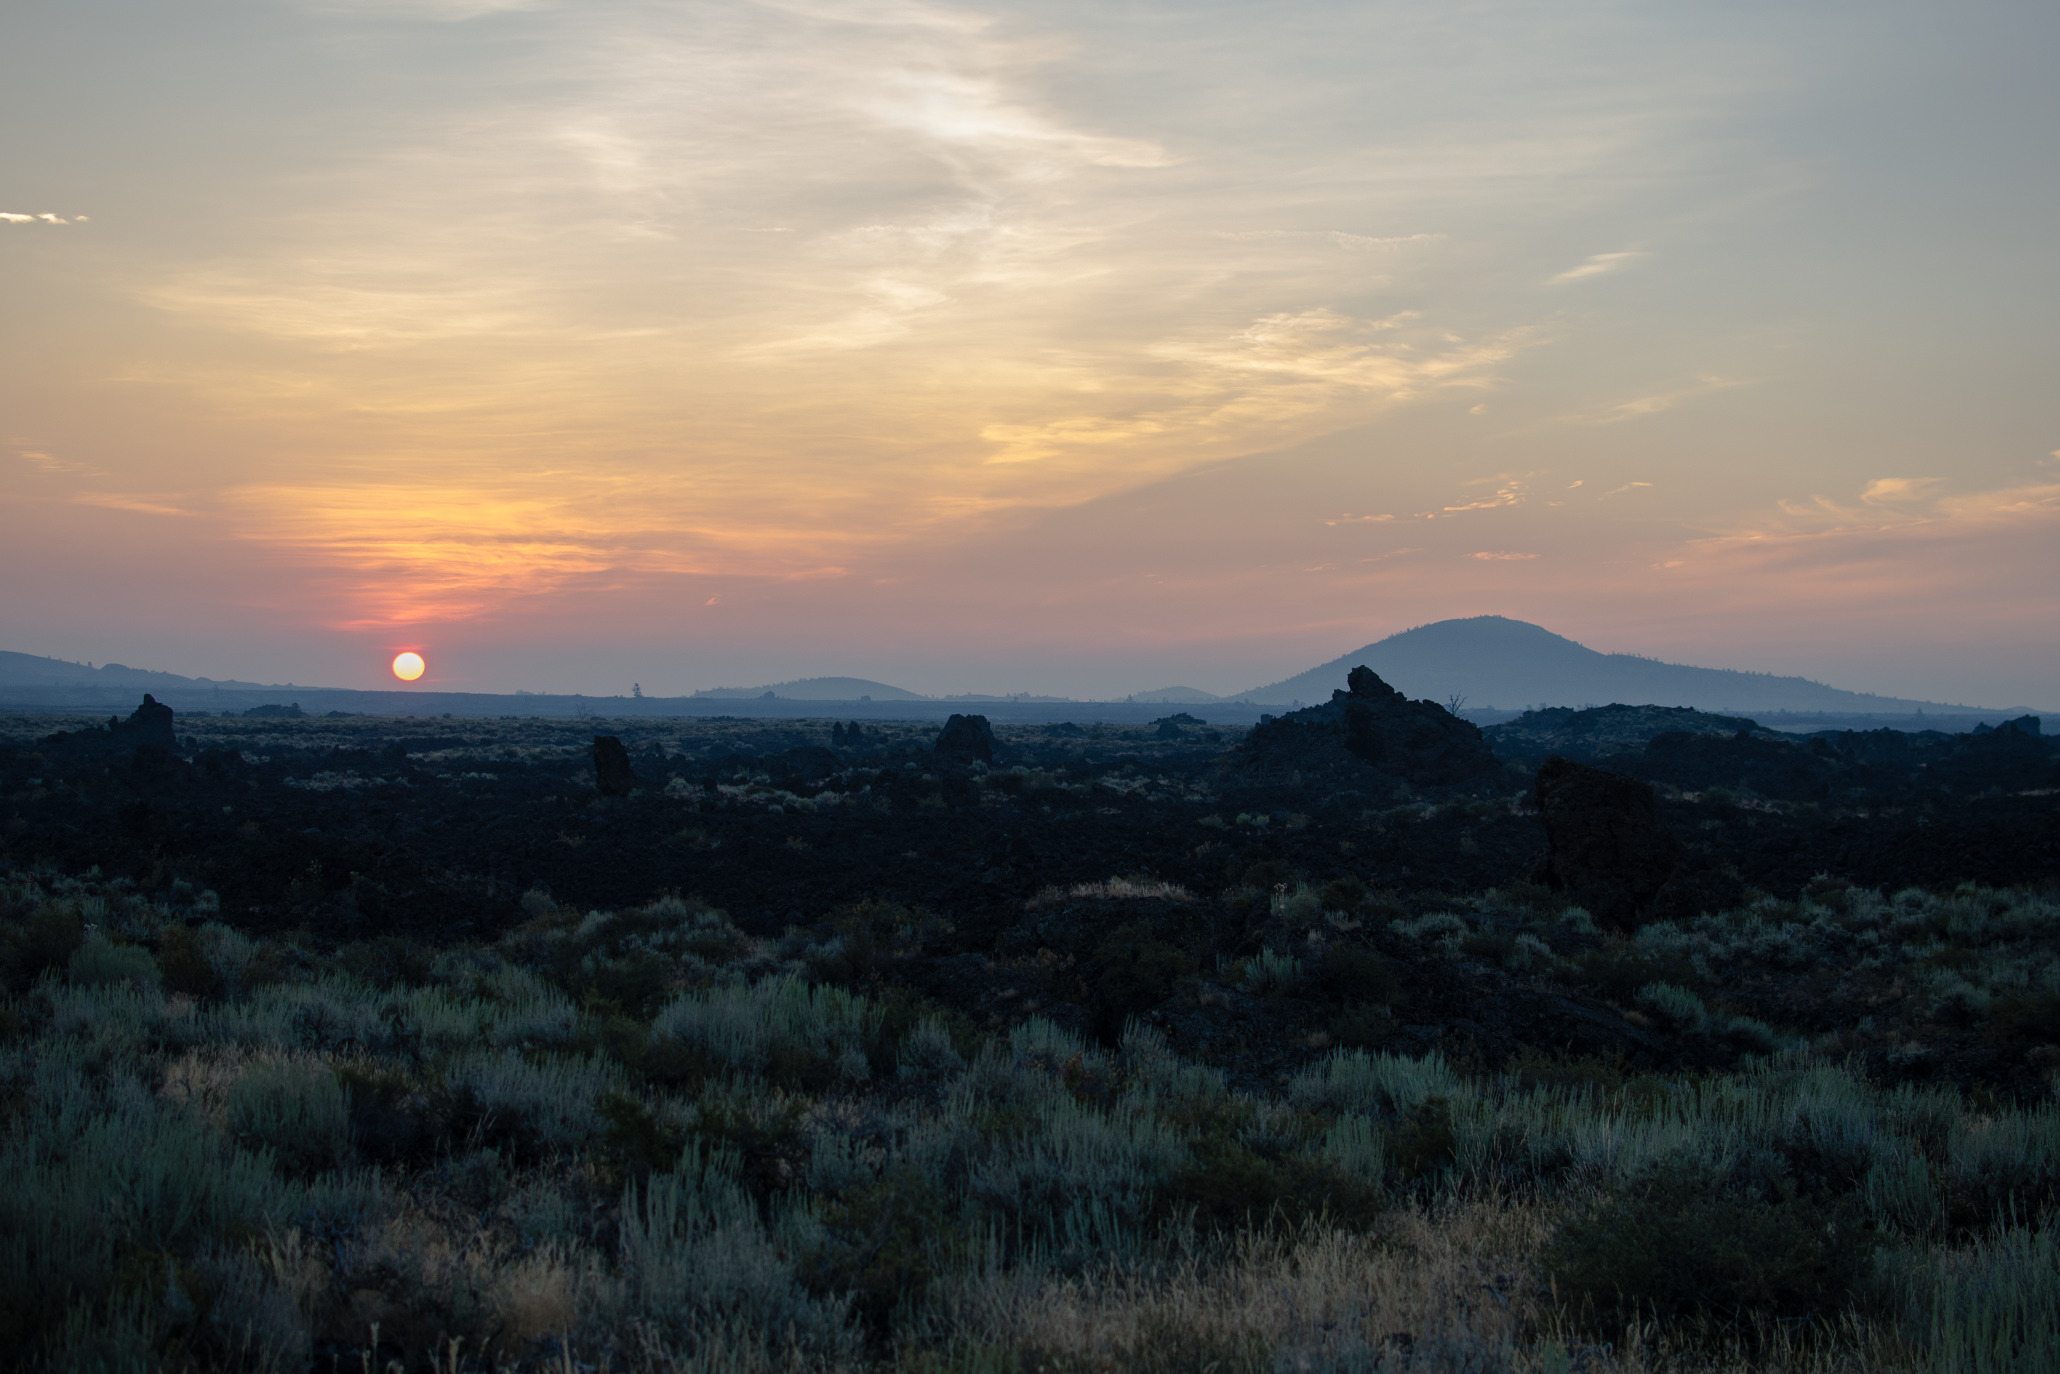
\includegraphics[width=0.50\textwidth]{sunrise-craters-of-the-moon.jpg}}
%\caption{We left Meridian at 4:00 am and headed east to Mackay Idaho to see the
%eclipse. On the way we caught the Sun rising over the Craters of the
%Moon. It was a good start to eclipse day.}
%\label{fig:5430x1}
%\end{figure}

\begin{SCfigure}
\centering
\href{https://conceptcontrol.smugmug.com/Places/USA-and-Canada/Idaho-Instants/i-mXNChFm/A}{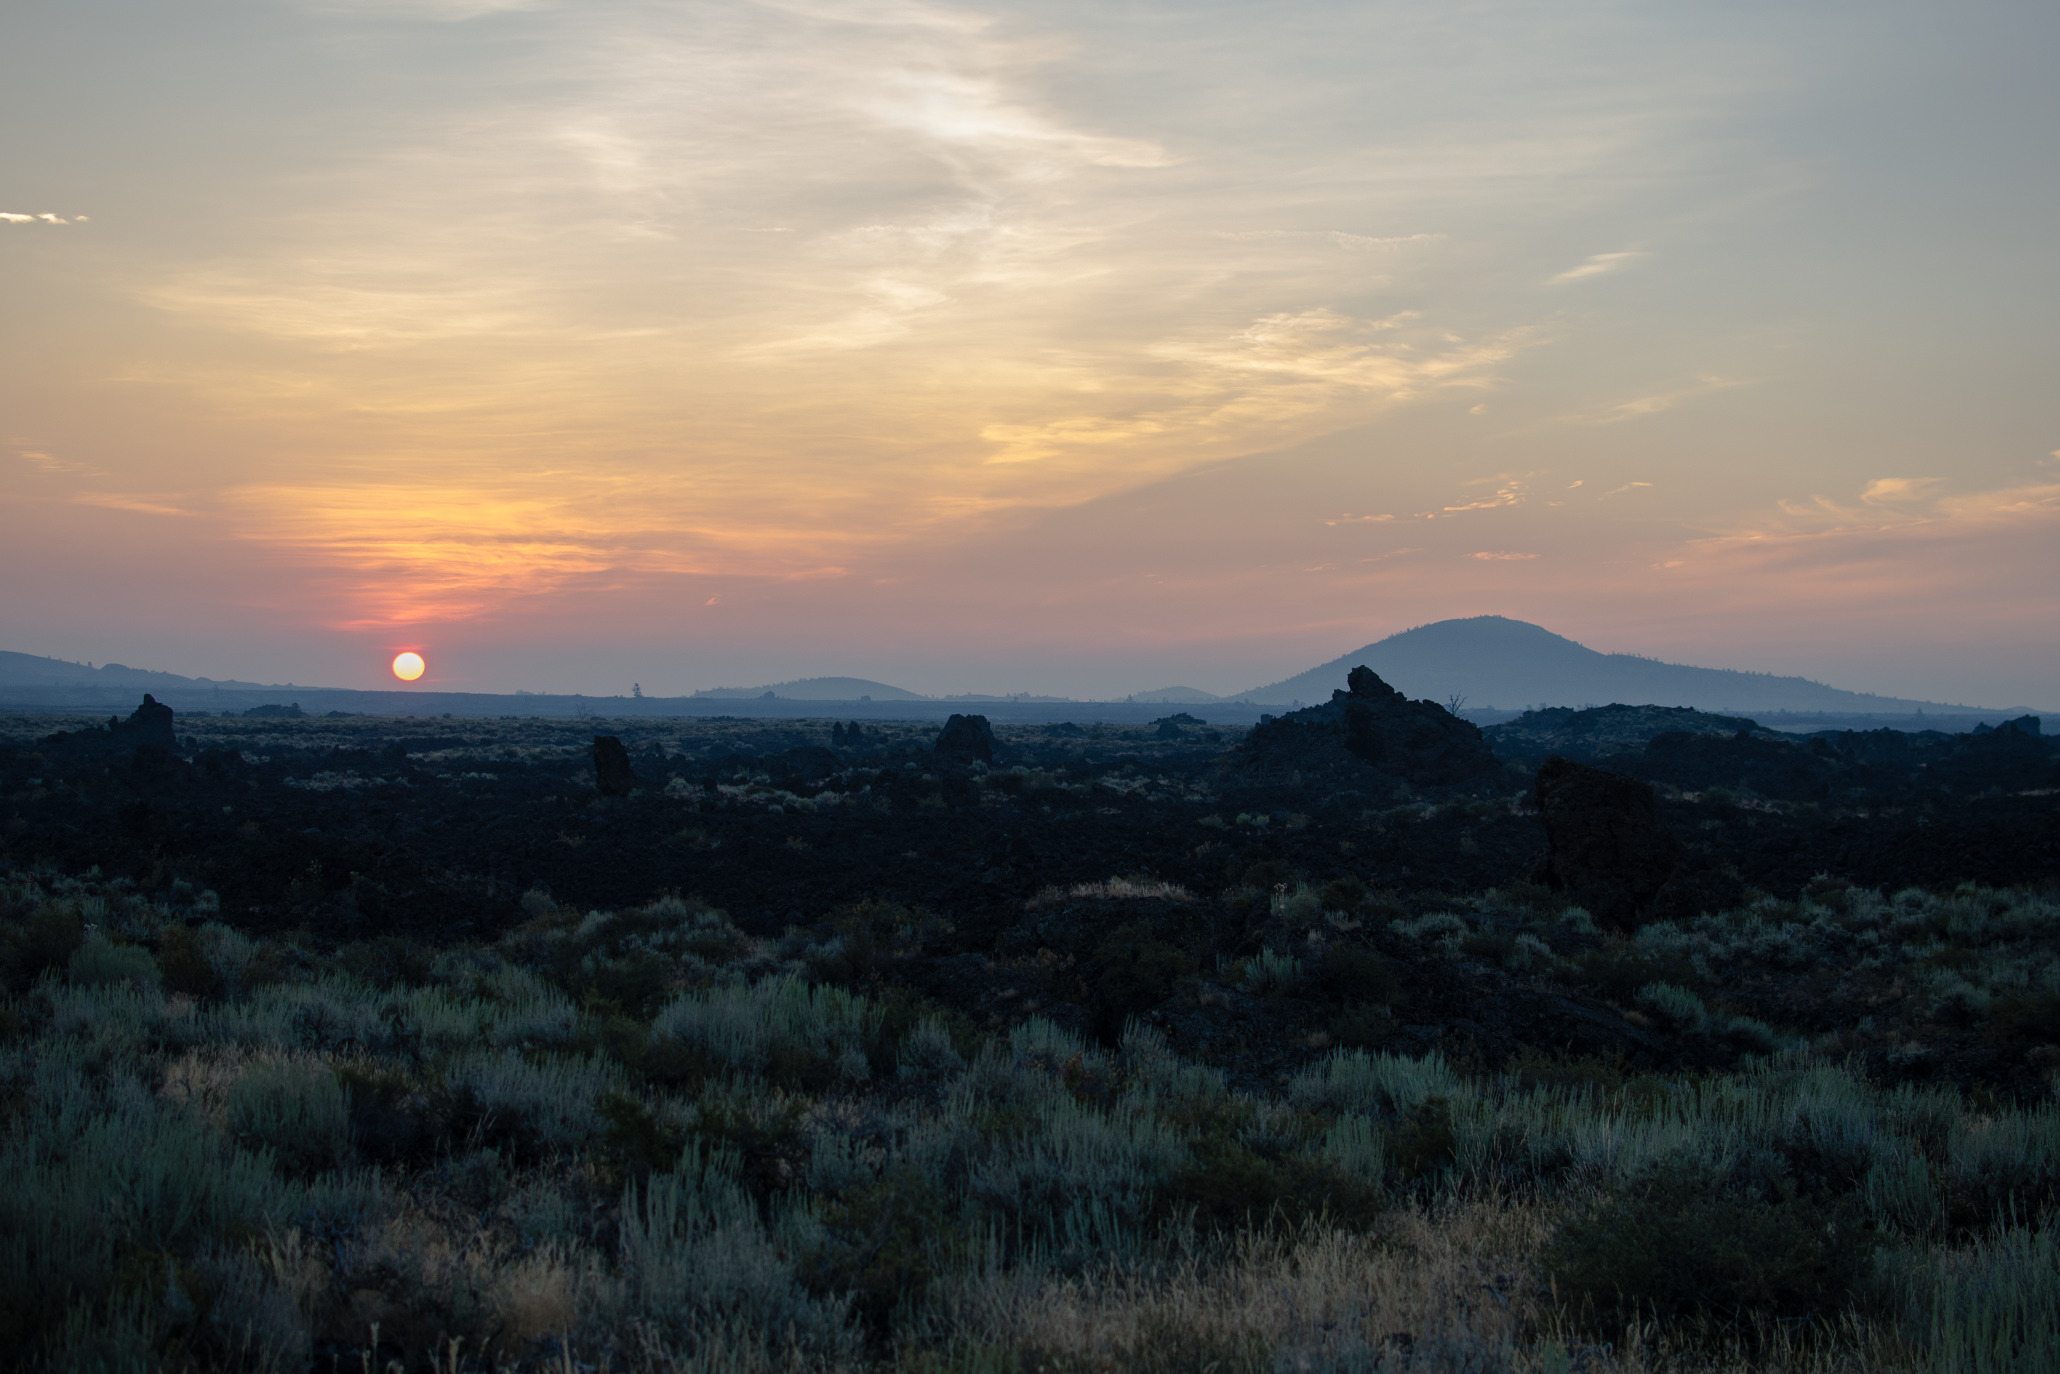
\includegraphics[width=0.5\textwidth]{sunrise-craters-of-the-moon.jpg}}
\caption{We left Meridian at 4:00 am and headed east to Mackay Idaho to see the
eclipse. On the way we caught the Sun rising over the Craters of the
Moon. It was a good start to eclipse day.}
\label{fig:5430x1}
\end{SCfigure}


Turning north at Arco Idaho we headed north to Mackay. There was more
smoke in the air than I would have liked. The further north we went the
thicker the smoke got. When we reached Mackay you could smell the smoke.
Mackay sits in a valley. Details on mountains to the east and west were
obscured by smoke but the sky was completely clear of clouds and at
totality the sun would be high overhead. I worried about smoke's impact
on the corona but I cheered myself up with the thought that sunblock
cream wouldn't be necessary.


%{[}caption id=``attachment\_5443'' align=``aligncenter''  width=``500''{]}
%\href{https://conceptcontrol.smugmug.com/Places/USA-and-Canada/Idaho-Instants/i-8P2mvsJ/A}{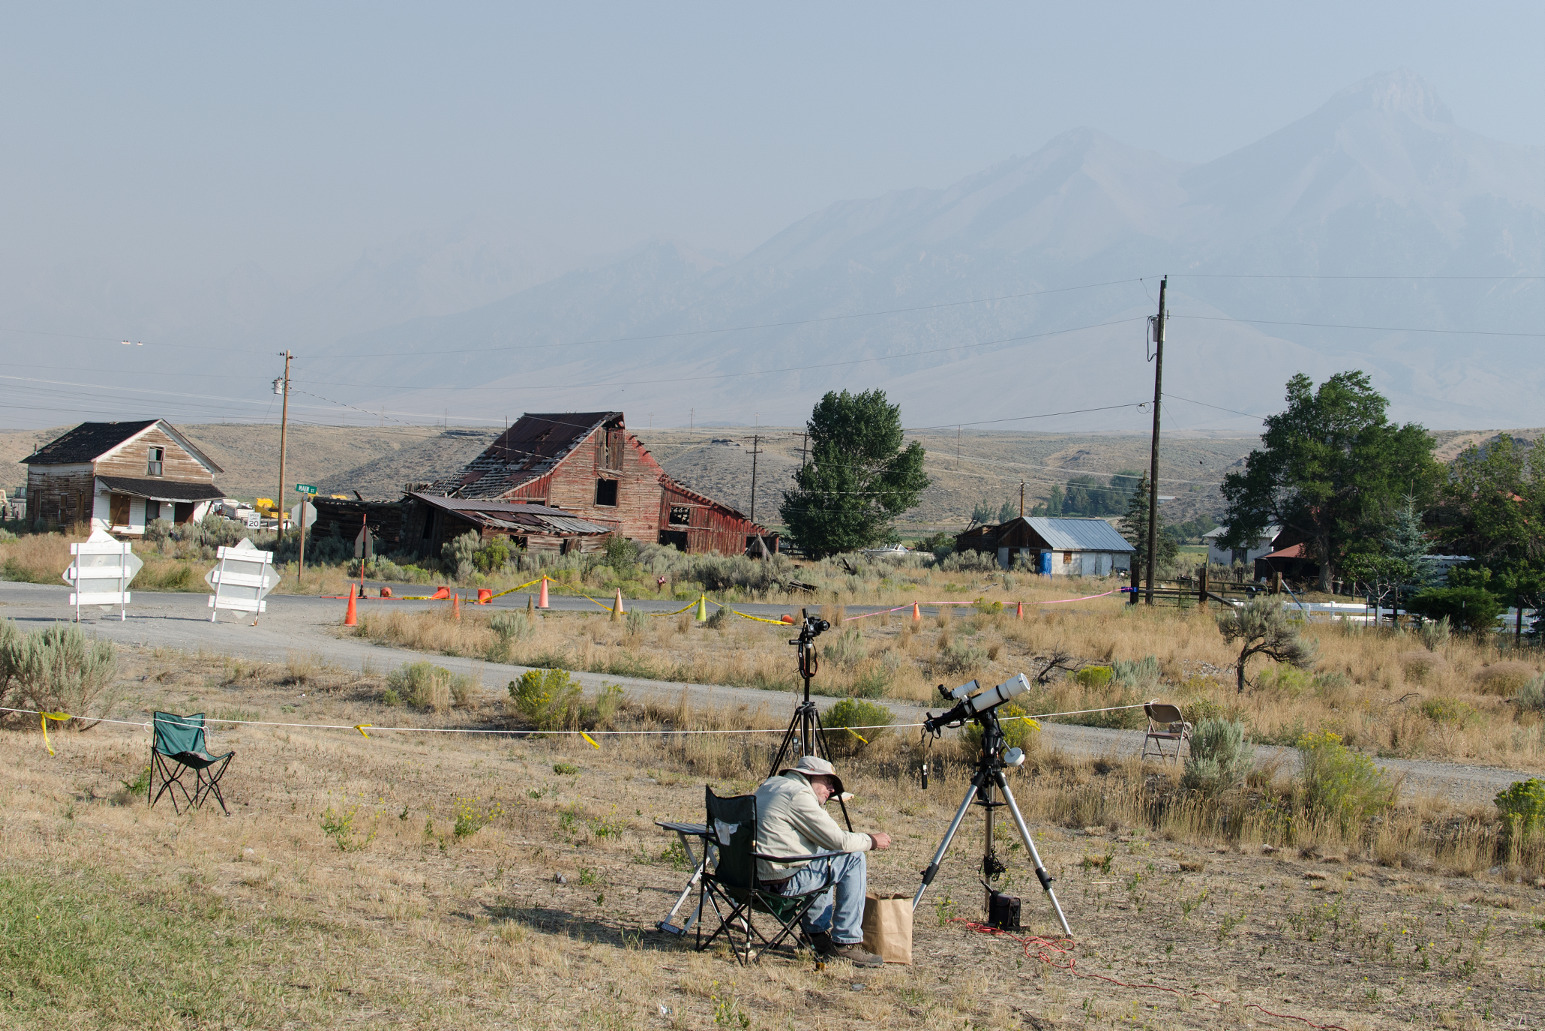
\includegraphics[width=5.20833in,height=3.47917in]{https://bakerjd99.files.wordpress.com/2017/08/getting-ready-totality-mackay.jpg?w=300}}
%Getting ready for totality. This shot shows how much forest fire smoke
%was in the air. The mountains of the Lost River Range are almost
%completely obscured in the background. The smoke probably reduced our
%view of the corona at totality but it increased the darkness and helped
%cast a deep orange red 360-degree dusk.
%{[}/caption{]}

%\begin{figure}[htbp]
%\centering
%\href{https://conceptcontrol.smugmug.com/Places/USA-and-Canada/Idaho-Instants/i-8P2mvsJ/A}{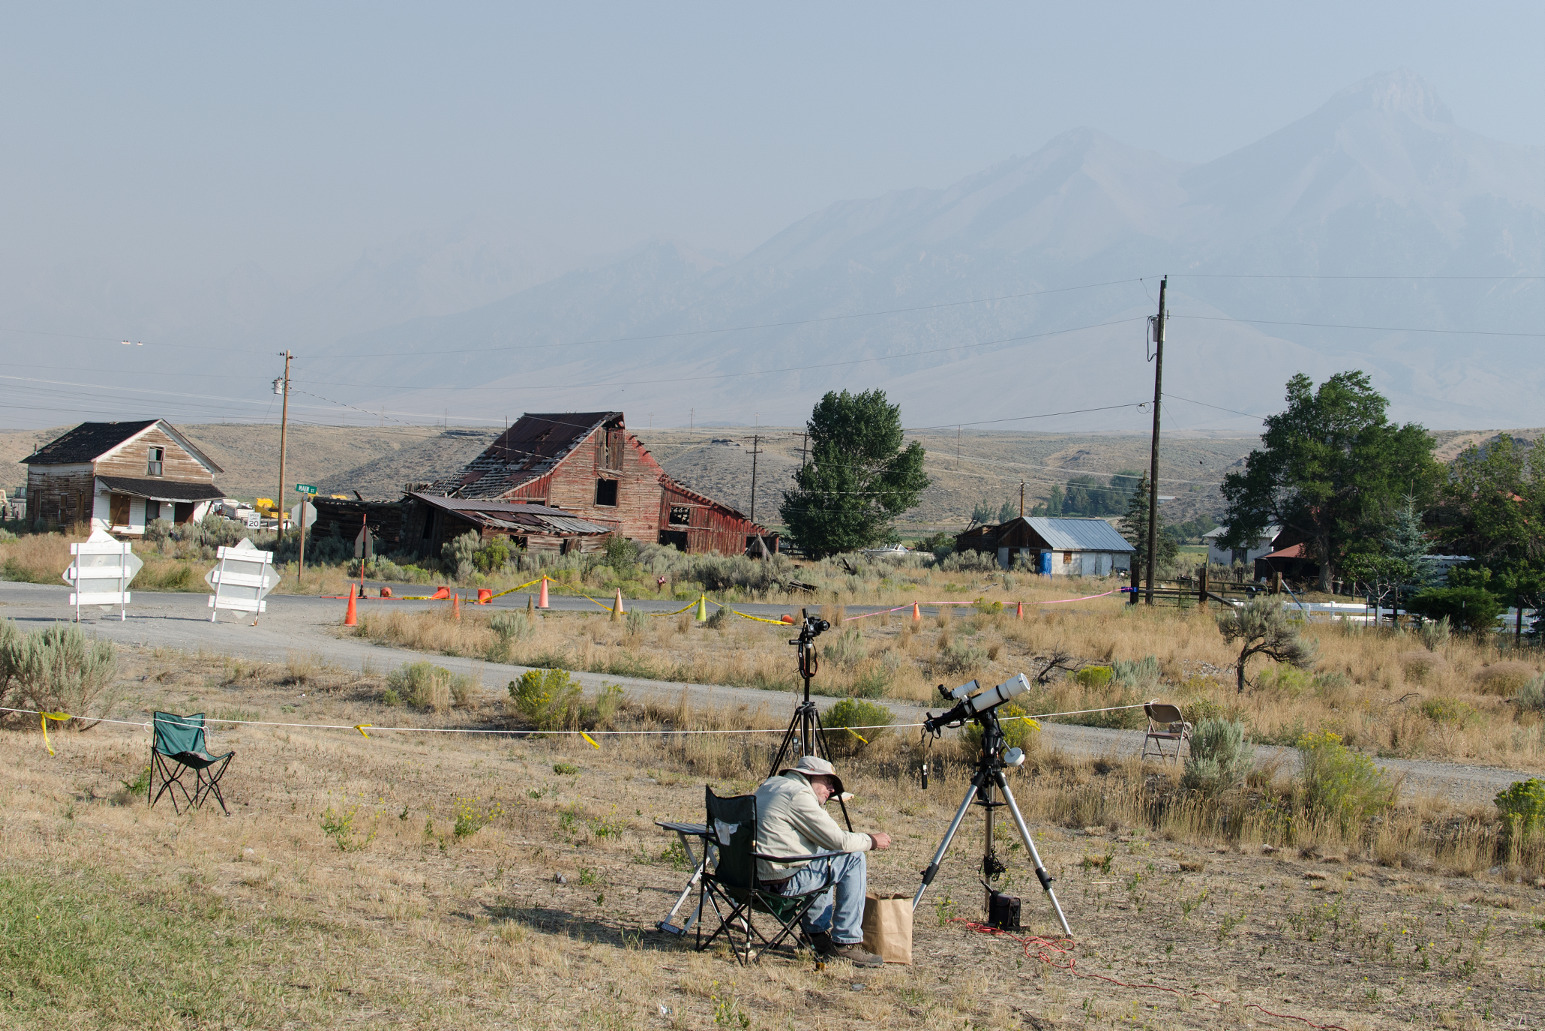
\includegraphics[width=0.50\textwidth]{getting-ready-totality-mackay.jpg}}
%\caption{Getting ready for totality. This shot shows how much forest fire smoke
%was in the air. The mountains of the Lost River Range are almost
%completely obscured in the background. The smoke probably reduced our
%view of the corona at totality but it increased the darkness and helped
%cast a deep orange red 360-degree dusk.}
%\label{fig:5430x2}
%\end{figure}

\begin{SCfigure}
\centering
\href{https://conceptcontrol.smugmug.com/Places/USA-and-Canada/Idaho-Instants/i-8P2mvsJ/A}{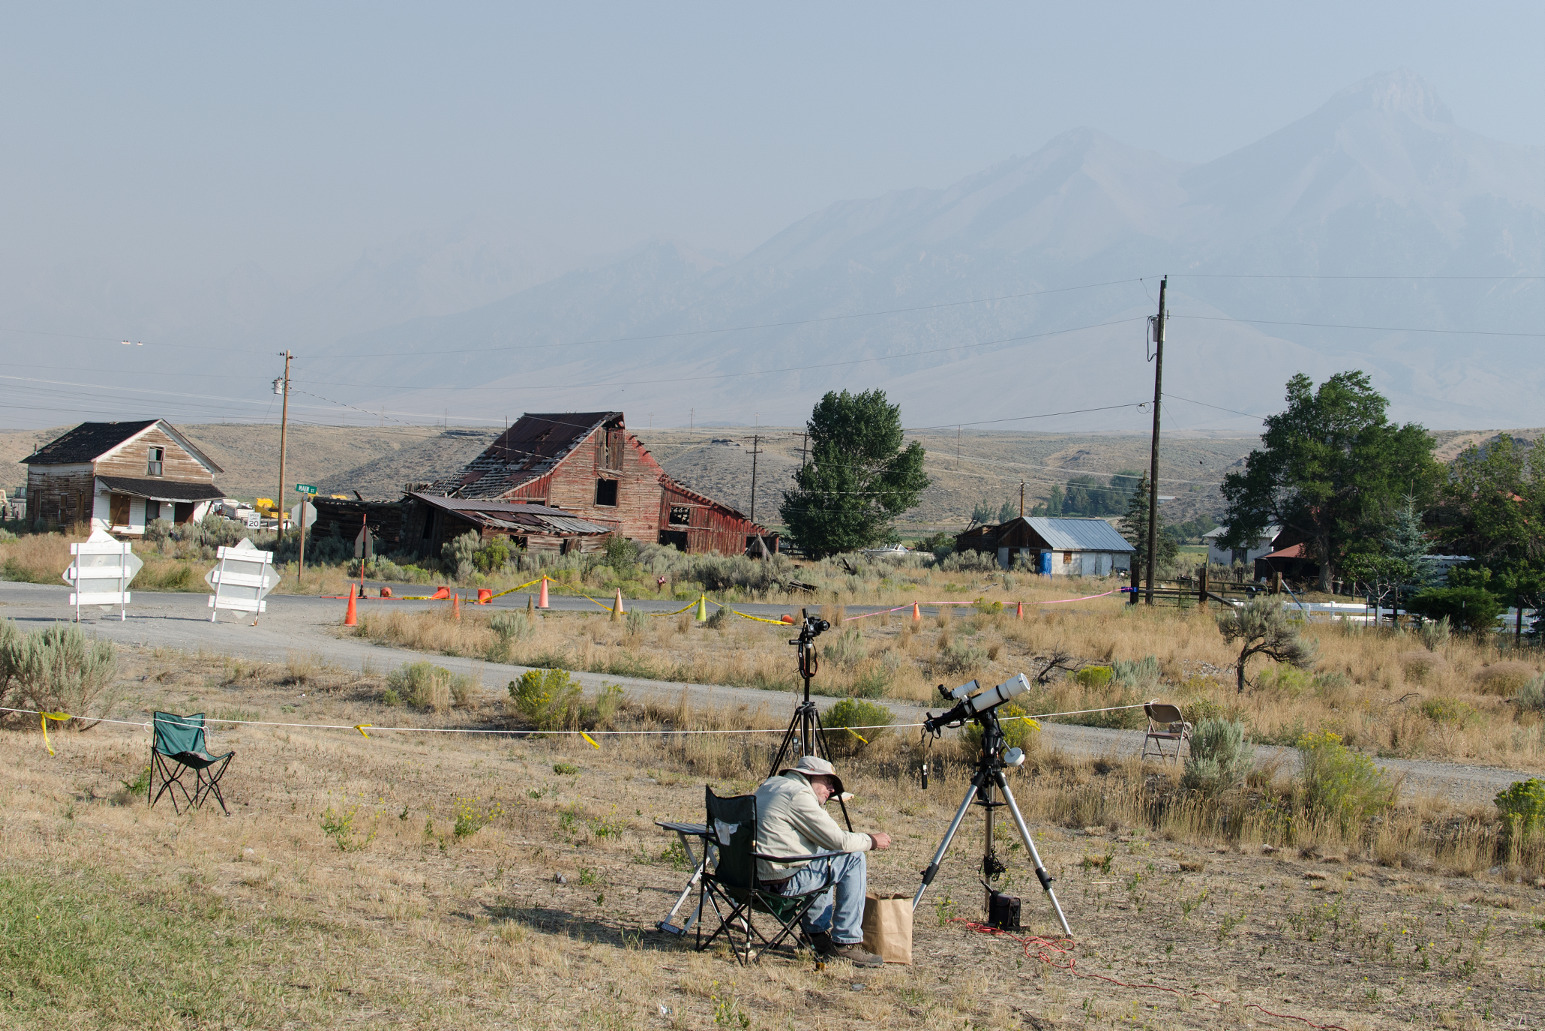
\includegraphics[width=0.50\textwidth]{getting-ready-totality-mackay.jpg}}
\caption{Getting ready for totality. This shot shows how much forest fire smoke
was in the air. The mountains of the Lost River Range are almost
completely obscured in the background. The smoke probably reduced our
view of the corona at totality but it increased the darkness and helped
cast a deep orange red 360-degree dusk.}
\label{fig:5430x2}
\end{SCfigure}
 


Being two hours early Mali decided to nap in the car while I walked
around Mackay taking pictures. Main Street was blocked off and street
vendors were setting up tented stalls and big meat smokers. Others were
busy selling souvenirs. Most of the stores were closed. The eclipse was
a good excuse for a holiday. I waited in a donut line and chatted with
other eclipse tourists. One Maryland couple had just arrived in a rented
car from Salt Lake City. A few Italians had come all the way from
Naples. I saw lots of Utah, California, Alberta and Nevada license
plates. Total solar eclipses gather the multitudes.


%{[}caption id=``attachment\_5439'' align=``aligncenter''  width=``500''{]}
%\href{https://conceptcontrol.smugmug.com/Places/USA-and-Canada/Idaho-Instants}{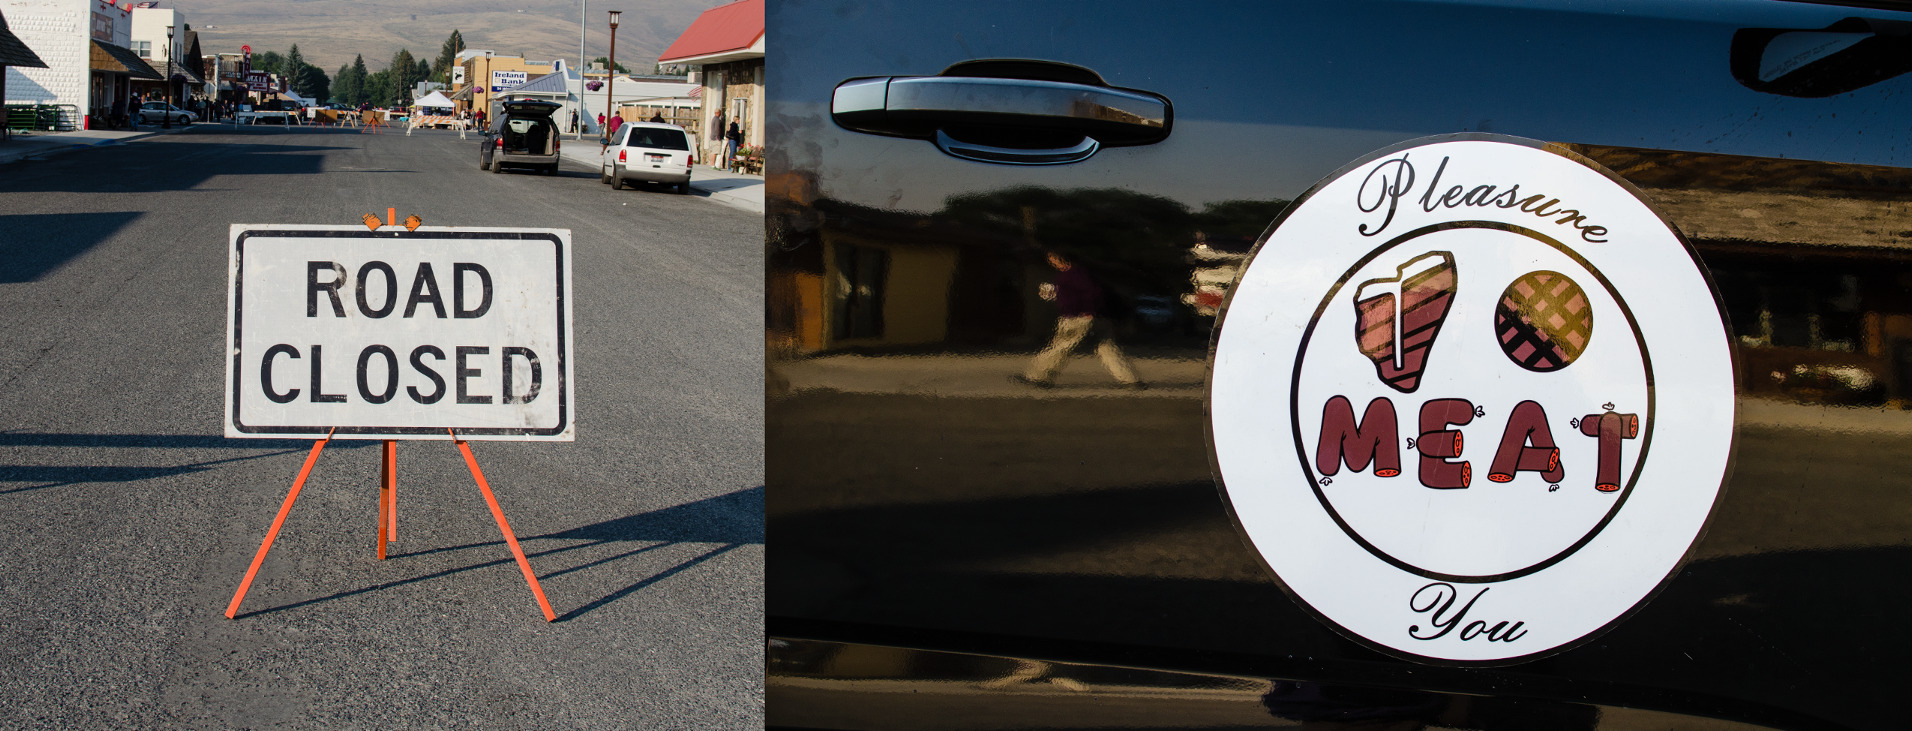
\includegraphics[width=5.20833in,height=1.98958in]{https://bakerjd99.files.wordpress.com/2017/08/mackay-eclipse-day.jpg?w=300}}
%Mackay blocked off Main Street for anticipated eclipse crowds. The
%number of people that showed up underwhelmed. The only eclipse
%complaints I am aware of were made by businesses hoping to cash in on
%massive crowds. Crowds were down over the entire country. Too many
%people were scared away by horror stories about traffic and the rest
%bought the malarkey that 99\% coverage is close enough to 100\%.
%Eclipses are not tests. That last 1\% obscures a vast unfathomable
%difference.
%{[}/caption{]}

\begin{figure}[htbp]
\centering
\href{https://conceptcontrol.smugmug.com/Places/USA-and-Canada/Idaho-Instants}{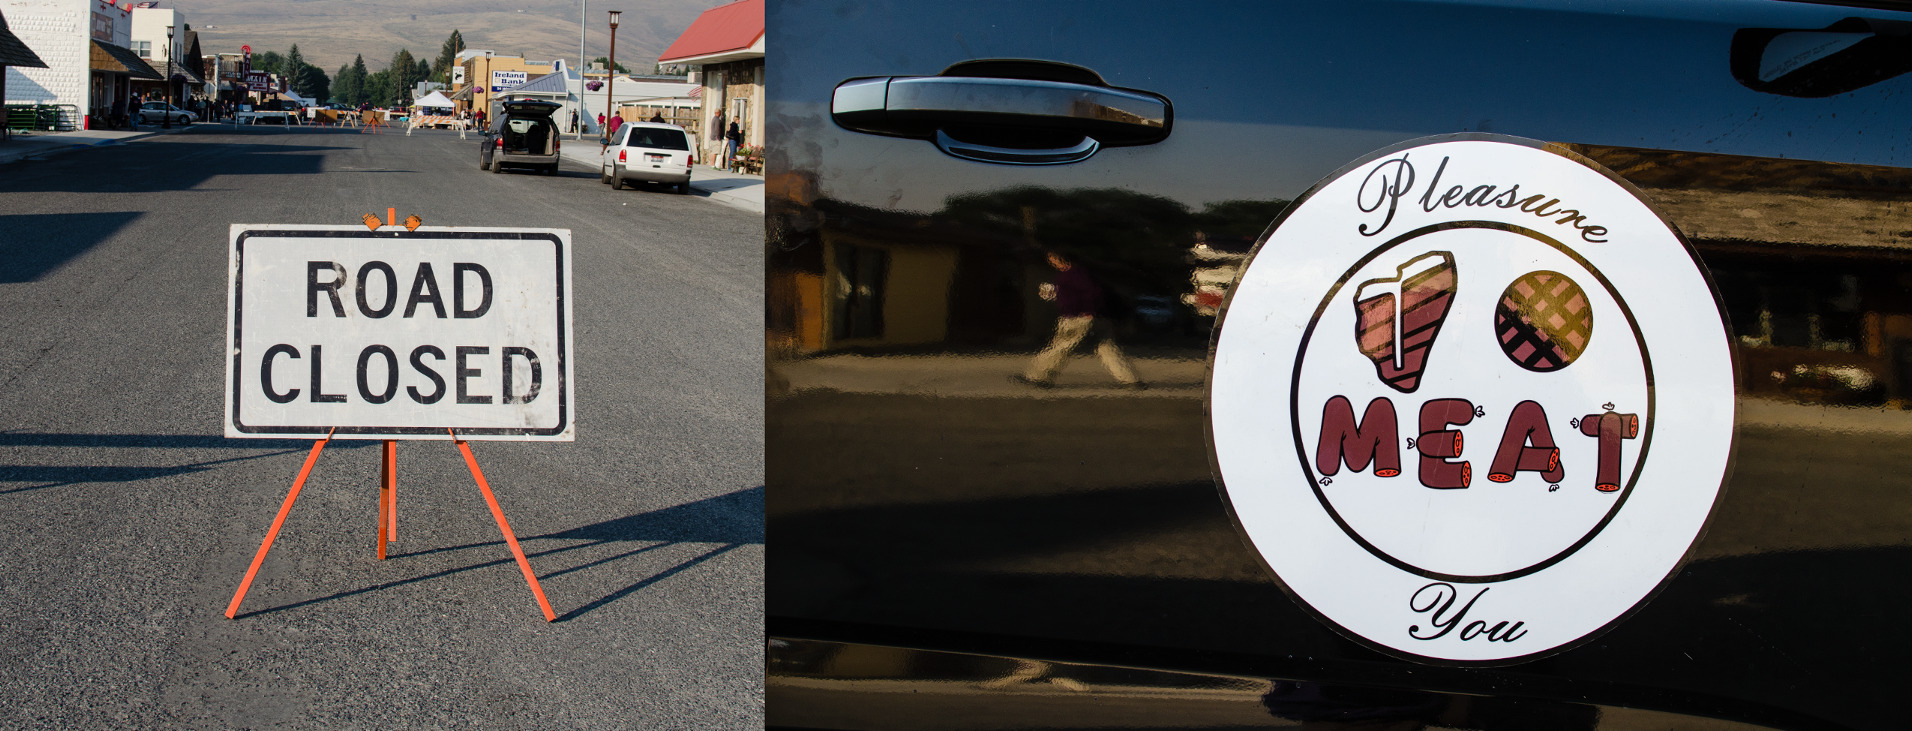
\includegraphics[width=0.75\textwidth]{mackay-eclipse-day.jpg}}
\caption{Mackay blocked off Main Street for anticipated eclipse crowds. The
number of people that showed up underwhelmed. The only eclipse
complaints I am aware of were made by businesses hoping to cash in on
massive crowds. Crowds were down over the entire country. Too many
people were scared away by horror stories about traffic and the rest
bought the malarkey that 99\% coverage is close enough to 100\%.
Eclipses are not tests. That last 1\% obscures a vast unfathomable
difference.}
\label{fig:5430x3}
\end{figure}

%\begin{SCfigure}
%\centering
%\href{https://conceptcontrol.smugmug.com/Places/USA-and-Canada/Idaho-Instants}{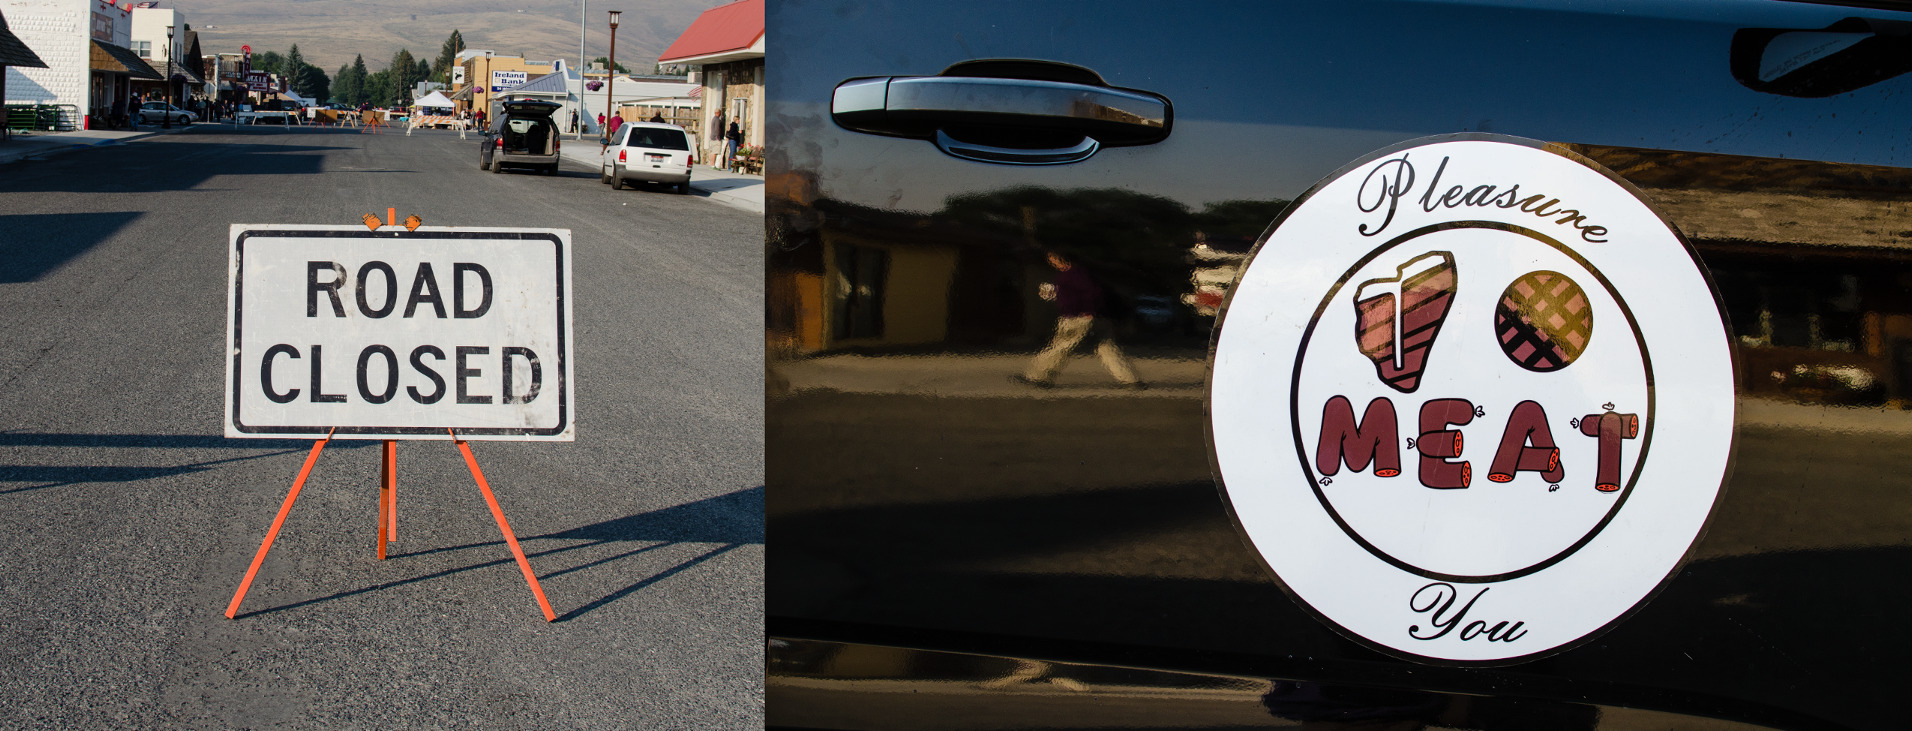
\includegraphics[width=0.5\textwidth]{mackay-eclipse-day.jpg}}
%\caption{Mackay blocked off Main Street for anticipated eclipse crowds. The
%number of people that showed up underwhelmed. The only eclipse
%complaints I am aware of were made by businesses hoping to cash in on
%massive crowds. Crowds were down over the entire country. Too many
%people were scared away by horror stories about traffic and the rest
%bought the malarkey that 99\% coverage is close enough to 100\%.
%Eclipses are not tests. That last 1\% obscures a vast unfathomable
%difference.}
%\label{fig:5430x3}
%\end{SCfigure}


After checking out downtown Mackay I drifted back to the Centennial Rest
Stop where Spanish science students were setting up equipment to observe
the eclipse. They had come all the way from Spain to watch the eclipse
in tiny Mackay Idaho. The moon's shadow turns even the most unlikely
places into tourist attractions. The scientific utility of total solar
eclipses in the 21\textsuperscript{st}~century is not what it used to be
but eclipses do offer great excuses for globe trekking and the
re-enactment of historical experiments. The Spaniards were busy
preparing weather balloons and getting ready to photograph the corona.
They were also making objective lens solar filters for people who
brought binoculars and telephoto lens. I considered having some made for
my 16x70 astronomical binoculars but decided against it. Instead, I went
back to our car, woke up Mali, and then started hauling eclipsing
paraphernalia to the viewing area. Unlike many present, we didn't have a
lot of gear: just binoculars, three-legged folding stools, cell phones,
cameras, and eclipse shades. Shortly after setting up our stools the
Spanish students started counting down to first contact. Shortly after
10:00 am the eclipse started.


%{[}caption id=``attachment\_5445'' align=``aligncenter''  width=``500''{]}
%\href{https://conceptcontrol.smugmug.com/Places/USA-and-Canada/Idaho-Instants/i-dGsRkQn/A}{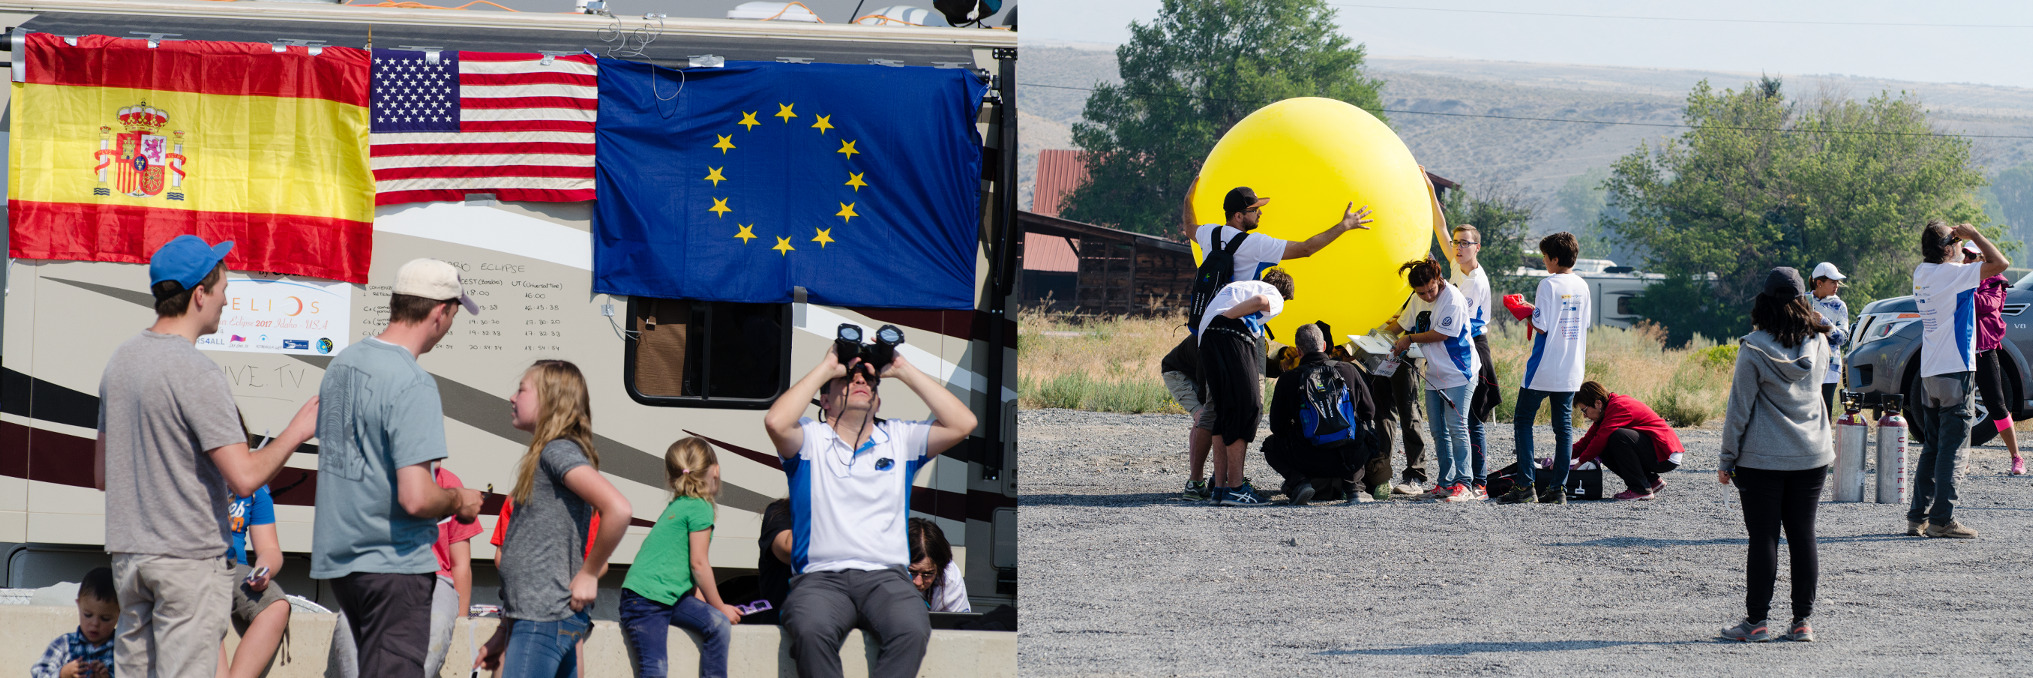
\includegraphics[width=5.20833in,height=1.73958in]{https://bakerjd99.files.wordpress.com/2017/08/spanish-ballon-van-flags.jpg?w=300}}
%A group of science students came all the way from Spain to watch the
%eclipse in Mackay Idaho. They brought a collection of telescopes, sun
%filters, and weather balloons. They released a balloon just before the
%eclipse, presumably to measure the eclipse induced temperature drop
%which was considerable. Mackay's elevation is almost 1800 meters. When
%the Sun goes down the temperature drops. The wind was blowing from the
%north and their balloon took off towards the south. They probably had a
%little road trip to recover it.
%{[}/caption{]}

\begin{figure}[htbp]
\centering
\href{https://conceptcontrol.smugmug.com/Places/USA-and-Canada/Idaho-Instants/i-dGsRkQn/A}{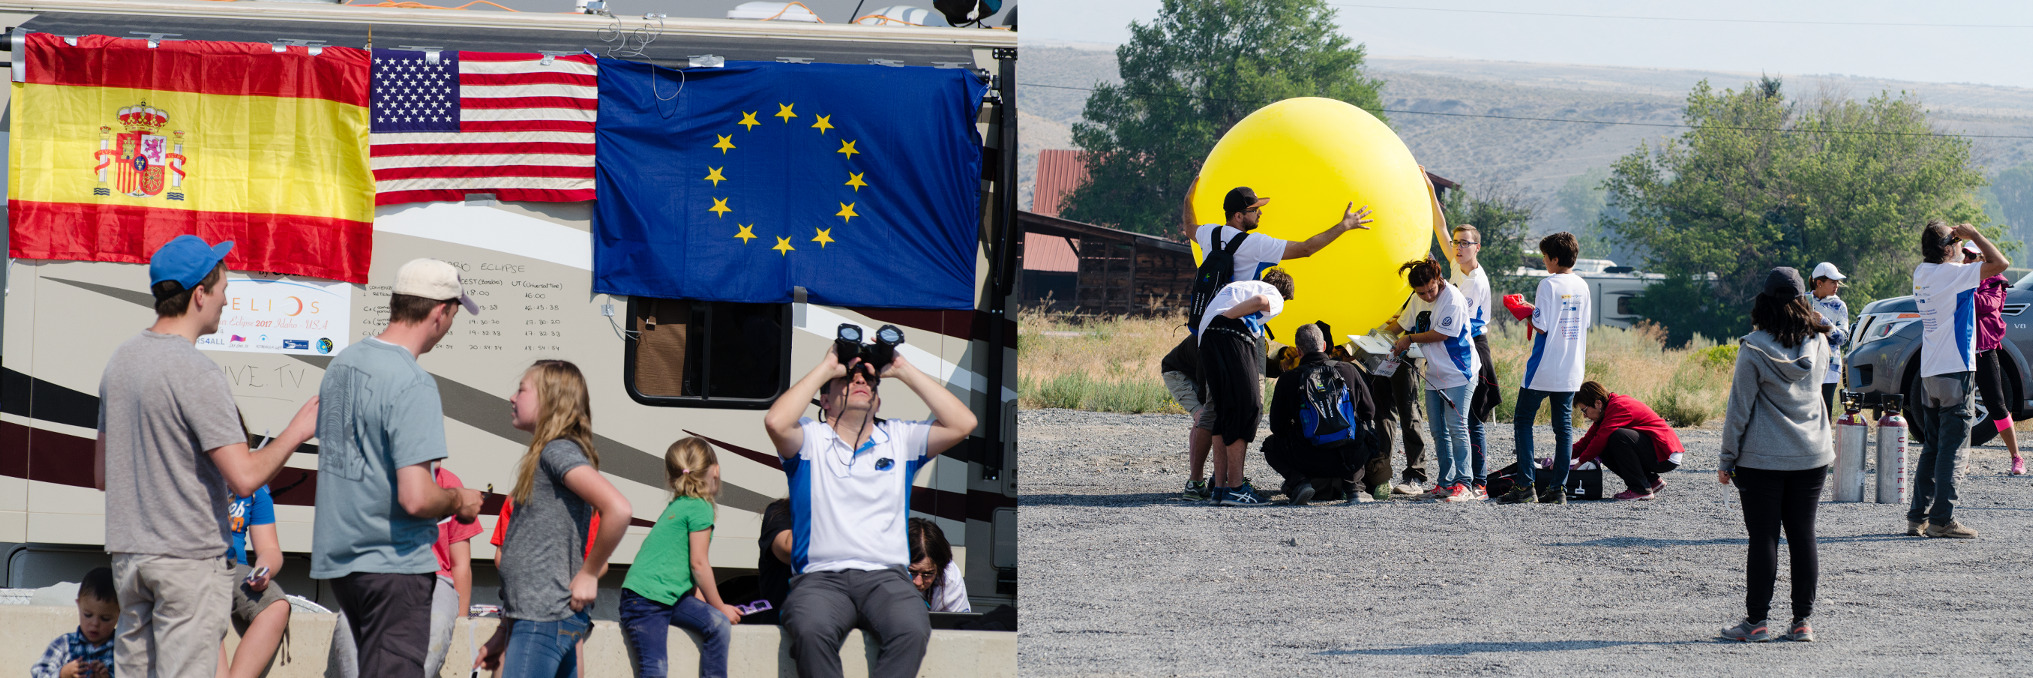
\includegraphics[width=0.75\textwidth]{spanish-ballon-van-flags.jpg}}
\caption{A group of science students came all the way from Spain to watch the
eclipse in Mackay Idaho. They brought a collection of telescopes, sun
filters, and weather balloons. They released a balloon just before the
eclipse, presumably to measure the eclipse induced temperature drop
which was considerable. Mackay's elevation is almost 1800 meters. When
the Sun goes down the temperature drops. The wind was blowing from the
north and their balloon took off towards the south. They probably had a
little road trip to recover it.}
\label{fig:5340x4}
\end{figure}

%\begin{SCfigure}
%\centering
%href{https://conceptcontrol.smugmug.com/Places/USA-and-Canada/Idaho-Instants/i-dGsRkQn/A}{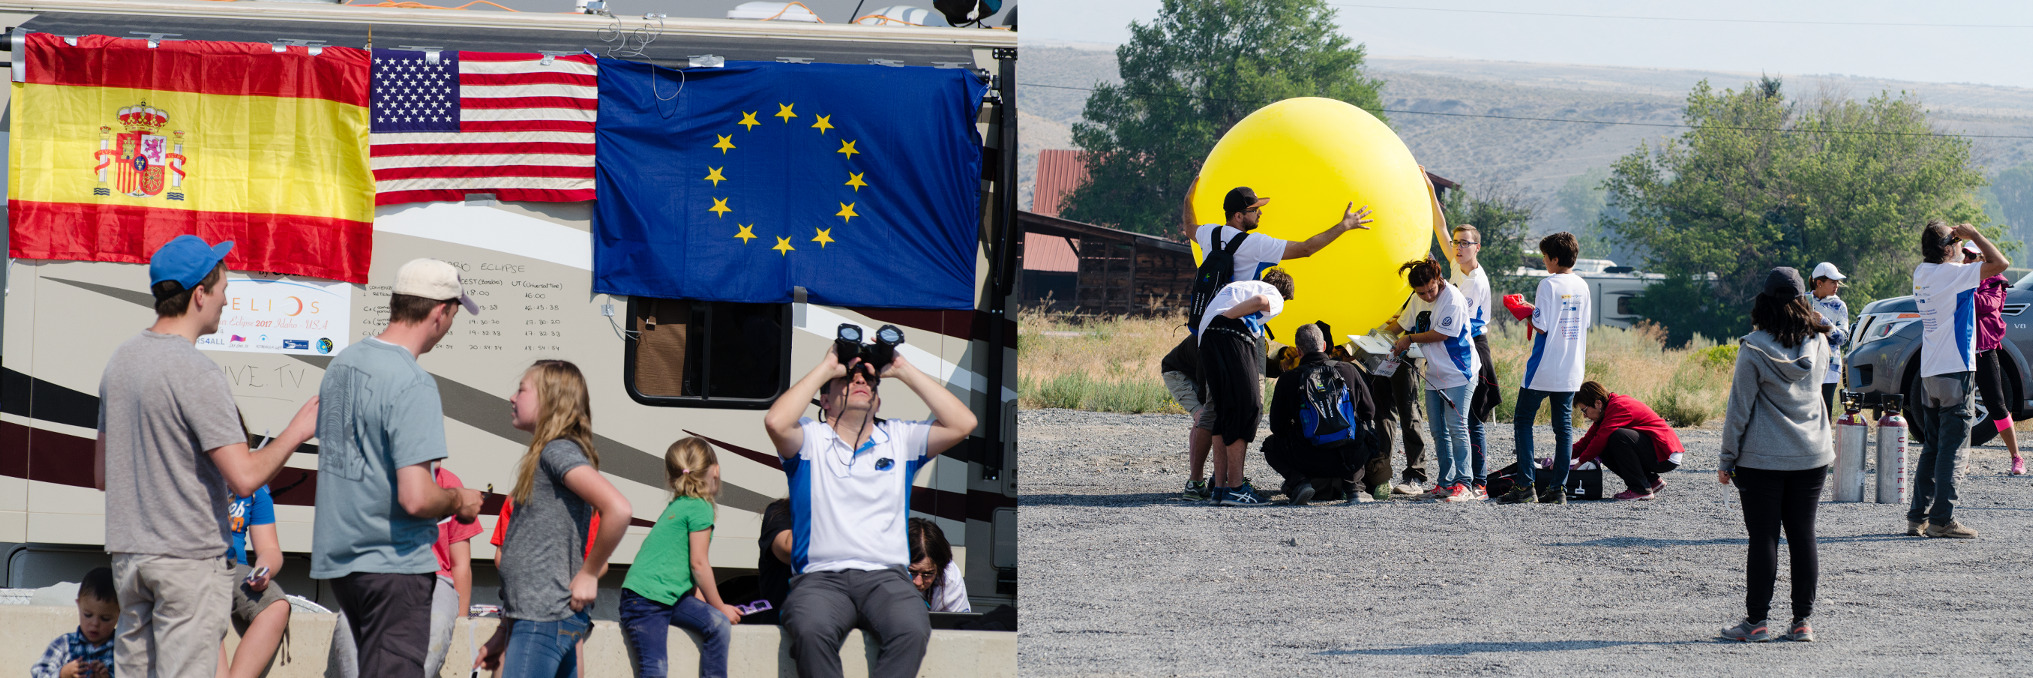
\includegraphics[width=0.5\textwidth]{spanish-ballon-van-flags.jpg}}
%\caption{A group of science students came all the way from Spain to watch the
%eclipse in Mackay Idaho. They brought a collection of telescopes, sun
%filters, and weather balloons. They released a balloon just before the
%eclipse, presumably to measure the eclipse induced temperature drop
%which was considerable. Mackay's elevation is almost 1800 meters. When
%the Sun goes down the temperature drops. The wind was blowing from the
%north and their balloon took off towards the south. They probably had a
%little road trip to recover it.}
%\label{fig:5430x4}
%\end{SCfigure}


At first, people were excited to see the Moon slowly nibble at the Sun's
disk but they quickly quieted down. I got the impression that many were
questioning the so-called awesomeness of solar eclipses. It's just a
boring black cookie-bite Sun. What's the big deal? I think many were
also surprised by how long it took for the Moon to cover the sun. I'd
seen this phase before so I wandered around the crowd taking pictures
while the Moon slowly covered the sun.

Fifteen minutes before totality the changing light was getting hard to
ignore. The human eye adapts logarithmically to changing light levels.
At this point in the eclipse more than 90\% of the sun was covered,
dropping light levels by a factor of ten, but it was only in the last
five minutes that it became obvious that it was getting dark. I spotted
a flock of pigeons gathering on the fences nearby. They were disturbed
by the change in routine. As totality approached people started counting
down. I peeled off my eclipse shades and glanced directly at the waning
light. As the sun squeezed down to a pinhole of brilliant light I saw
dazzling rainbow halos around the sun. I'm developing cataracts. When I
stare into bright point sources I see rainbow halos. I had never looked
at a point source as bright as the Sun and the effect was both beautiful
and alarming. I will have to do something about my cataracts in a few
years.


At totality, the blasé crowd erupted. Many started squealing, pointing,
and yelling. Mali pointed to a flock of pigeons, the same flock I had
spotted on the fence before, tearing through the air. I briefly looked
all around to see the 360-degree sunset. I was expecting a deep orange
dusk all around up but it failed to appear. We were too close to the
mountains. Then I pointed my 16x70 binoculars at the eclipsed sun. Three
flares were visible and the corona's filaments were as beautiful as
ever. The corona was not as extensive as the 2001 eclipse and the core
region near the sun seemed brighter. I looked around for planets and
stars. Venus was easy. I was expecting to spot Mercury and Mars but I
the only star I saw near the Sun I later identified as Regulus. I didn't
try to photograph my first total solar eclipse but near the end of
totality I grabbed my DSLR and fired off a few 300mm telephoto shots
just to see what might come up.


%{[}caption id=``attachment\_5447'' align=``aligncenter''  width=``400''{]}
%\href{https://conceptcontrol.smugmug.com/Places/USA-and-Canada/Idaho-Instants/i-25dfJkS/A}{\includegraphics[width=4.16667in,height=4.16667in]{https://bakerjd99.files.wordpress.com/2017/08/aug-21-2017-eclipse-corona1.jpg?w=300}}
%I didn't try and photograph my first total solar eclipse but this time I
%fired off a few 300mm handheld telephoto shots just to see what might
%come up. The result was better than I expected.
%{[}/caption{]}
%
%\begin{figure}[htbp]
%\centering
%\href{https://conceptcontrol.smugmug.com/Places/USA-and-Canada/Idaho-Instants/i-25dfJkS/A}{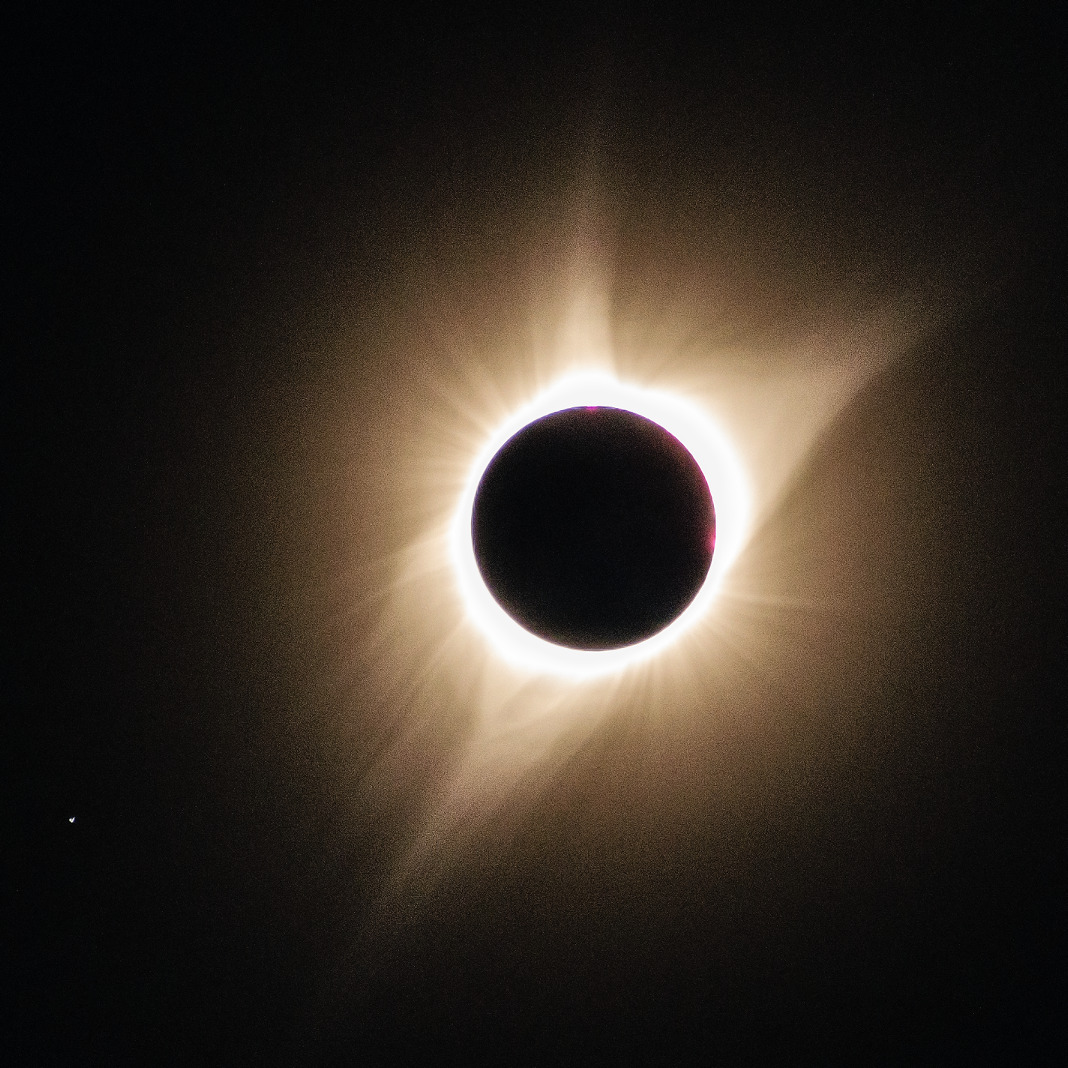
\includegraphics[width=0.4\textwidth]{aug-21-2017-eclipse-corona.jpg}}
%\caption{I didn't try and photograph my first total solar eclipse but this time I
%fired off a few 300mm handheld telephoto shots just to see what might
%come up. The result was better than I expected.}
%\label{fig:5340x5}
%\end{figure}

 \begin{SCfigure} 
 \centering
\href{https://conceptcontrol.smugmug.com/Places/USA-and-Canada/Idaho-Instants/i-25dfJkS/A}{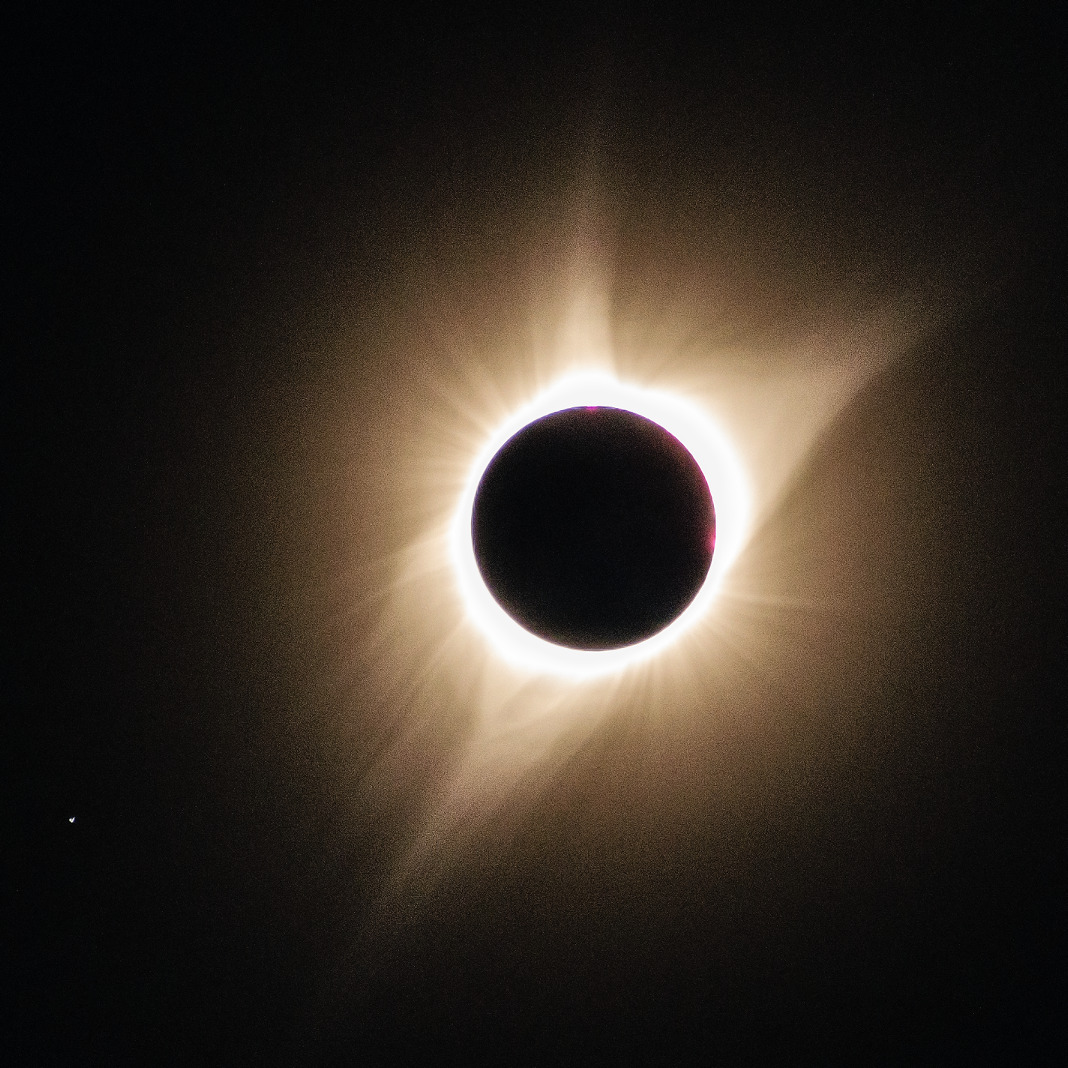
\includegraphics[width=0.4\textwidth]{aug-21-2017-eclipse-corona.jpg}}
 \caption{I didn't try and photograph my first total solar eclipse but this time I
fired off a few 300mm handheld telephoto shots just to see what might
come up. The result was better than I expected.}
 \label{fig:5340x5}
 \end{SCfigure}


Then, as suddenly as it started, the Sun burst forth. One bystander
yelled, ``Do it again!'' The small crowd kept buzzing as more of the Sun
was exposed. The consensus was, ``Yeah, total solar eclipses are
freaking awesome and totality is totally worth seeing.'' Later, while
standing in line to view the Sun and receding Moon through a Hydrogen
Alpha filtered telescope, I overheard a fellow in the crowd say, ``I'd
read about shadow chasers, people who go all over the world to see total
eclipses, I thought that was crazy, until today!''

The next total solar eclipse is in 2019. The greatest eclipse is in the
Pacific, later the shadow runs over parts of Chile and Argentina. I've
always wanted to visit the large observatories in Chile and view the
southern sky from the super dark high elevation skies of the Atacama.
This with totality is close to amateur astronomer heaven.



%\end{document}
 
% standard floating figure
% \captionsetup[figure]{labelformat=empty}
% \begin{figure}[htbp]
% \centering
% \href{}{\includegraphics[width=0.50\textwidth]{}}
% \caption{}
% \label{fig:????x0}
% \end{figure}
 
% captions beside figure
% \captionsetup[figure]{labelformat=empty}
% \begin{SCfigure}
% \centering
% \href{}{\includegraphics[width=0.40\textwidth]{}}
% \caption{}
% \label{fig:????x0}
% \end{SCfigure}
 
% wrapped figure - outer size > inner size
% \captionsetup[floatingfigure]{labelformat=empty}
% \begin{floatingfigure}[l]{0.23\textwidth}
% \centering
% \href{}{\includegraphics[width=0.22\textwidth]{}}
% \caption{}
% \label{fig:????x0}
% \end{floatingfigure}
